% vim: tw=80 et sw=4
\documentclass{sydeStyle}
\usepackage{amsmath}
\usepackage{amssymb}
% \usepackage{graphicx}
\usepackage{longtable}
\usepackage{nameref}
\usepackage{subfig}
\usepackage[xindy,toc,style=long3col]{glossaries}

\newglossary[slg]{symbol}{sym}{sbl}{List of Symbols}
\makeglossaries

\DeclareGraphicsExtensions{.eps}

\coursecode{462}
\prof{Professor Stashuk}
\title{
Design of an Autonomous Hang-Glider Controller - Final Report
}
\date{\today}

\author{Andrew Cameron, 20252410}
\authorthree{Peter Lobsinger, 20195824}

\begin{document}
%TODO: describe all symbols, possibly in a Table of Symbols.

\maketitle

\tableofcontents

\chapter{Introduction}
% This should introduce the topic in a manner understandable by anyone with a
% reasonable technical background (i.e. any 1st year engineering student should
% be able to understand the problem). Identify the need or problem that you want
% to address and why you want to address it. Indicate why and to whom the
% problem is important.  Background information should motivate the need for the
% design and show the nature, extent or significance of the problem you have
% defined.  This can be done, for example, by identifying inadequacies in
% existing designs, demonstrating an industry need for such an implementation,
% or reviewing existing research on the topic.  These three aspects
% (Introduction, Background and Problem Statement) can be organized in separate
% sections, or all together, etc. in order to suit the readability for your
% particular workshop.

The competition in which the Waterloo Rocketry Team (WRT) aims to compete has a
component of the score determined by functionality and innovation of the
payload\cite{IREC}. The WRT spawned several payload projects with the aim of
achieving a good standing in this category. One such project was a
rocket-deployed glider, which launches at apogee.

The preferred design for the glider was the Parasev. A Parasev consists of a
wing suspending a control mass\cite{wiki:parasev}. The wing is a high-sweepback
delta wing composed of sailcloth held loosely to a frame which defines the
leading edges and a central keel. The craft is navigated by positioning the wing
at an offset from the control mass, generating moments which change the craft's
orientation.

4A Mechanical Engineering student, Gandhali Joshi, undertook the mechanical
design of this glider as her fourth year design project. The control of the
craft, however, was not a component of this project.

All components of the rocket and payload must be recovered within a 2 hour
window. Teams failing to comply with this regulation face disqualification from
the competition \cite{IREC}. This project was undertaken to design a control
system for this glider that would facilitate the recovery of the craft.

\chapter{Objectives}
\label{sec:objs}
% The objectives should not have changed in principle from the Design Plan and
% Interim Report, however, you may want to rework them to ensure that they fit
% in with the rest of the report.  Do not discuss why objectives may have been
% reworked here; this should be saved for the “Description of Time-Line” section
% (described below).

The launch of the glider from the rocket is the responsibility of the rocketry
team. The glider will be launched to a state that is suitable for flight and
clear of all components of the rocket.

\section{Maintain Flight}
\label{sec:obj1}

The control system must ensure that the craft remains in stable flight through
the duration of its control, that is, from the end of the glider launch sequence
to the landing. To ensure the requirement is reasonable attainable, it does not
require the consideration of meteorological conditions. It can be assumed that
the craft flies through windless, constant-density air.

\section{Fly to Target}
\label{sec:obj2}

In order to make recovery as convenient as possible, the primary objective of
the craft's control system is to arrive at a predetermined point on the ground,
specifically, the launch area, or a neighbouring location.

This objective is only feasible for a range of initial conditions. Fortunately,
the rocket launch provides a relatively narrow range of initial conditions. The
apex of the flights of the rocket under consideration will range from between
2~km and 5~km above ground level, with lateral displacement less than 1~km. Up
to 1~s of freefall before deployment gives 0~m/s to 9.8~m/s initial downward
velocity. Between 0.5~m/s and 3~m/s lateral speed are expected at the apex of
the rocket's flight, and are therefore the initial condition's ground speed
range. The assumption that the deployment procedure will position the craft in
a state favourable to flight can be formalized to an orientation that gives
between 0 and 30 degrees angle of attack, no sideslip, and zero angle rates.

\section{Land Safely}

Recoverability and reusability, important objectives for the WRT, depend heavily
on a graceful landing. Moderate impact shocks are acceptable for an unmanned
craft designed with rough landings in mind. The control system will arrange for
the craft to hit the ground within acceptable bounds for the designed glider.

\chapter{Methodology}
% Criteria (measurable qualities) and constraints (hard decisions) should be
% provided to guide the design process and motivate preferred solutions.  The
% extent of the use of criteria and constraints is project dependent.  The
% design group should provide sufficient information in this section to fully
% justify the methods used.

\section{Modelling of Craft Dynamics}
\label{sec:modelling}
% Since you model lift and drag forces and so on, it's my understanding that it
% counts as 'dynamics'.  But you're the expert, so if you want to change the
% title, that's your prerogative! =)

In order to gain insight into craft behaviour and to evaluate controller
performance, a model of the dynamics of the craft was created based on existing
work \cite{Rogallo1960}\cite{Layton1963}\cite{spottiswoode}. A set of simulation
and visualization software tools were created based on this model.

\subsection{Simplifying Assumptions}

In order to create a simple model demonstrating the interesting, long-term
behaviour of the craft, a number of simplifications were made.

The craft was modelled as a single body, about the center of mass of the overall
system. This eliminates the requirement of considering forces internal to the
system, reducing the number of forces needing consideration. However, not
considering internal forces does entail neglecting some components of the
dynamics, leading to further assumptions being forced.

The control mass is assumed to move instantaneously to any commanded position.
This is clearly not physical, however, the control mass is moved using torques
at the hang point, which are some of the internal forces that have been omitted
from the model due to the single-body assumption. Due to the smoothness of
flight of real craft resembling the one being modelled, it is expected that the
control mass will be moved slowly and that, under these slow actuation
conditions, a real motor would be able to accomplish the desired position nearly
instantly, as compared to other aspects of the craft dynamics.

Another result of not modelling the control torques moving the control mass is
that the accelerations due to these cannot be modelled. This means that changes
in control mass position do not result in changes in wing orientation, as would
normally occur in a real craft. This unmodelled effect results in slight
transients in wing position response to control inputs. To the controller, this
unanticipated effect is simply another disturbance, and a controller designed
with disturbance rejection in mind will be more than capable of coping.

The inertia tensor is assumed to be fixed. In truth, movement of the control
mass changes the relative positioning of the masses of the system, resulting in
changes to the inertia tensor. Such changes affect the absolute and relative
magnitudes of the effect of external forces on the angle-rates of the craft.
Further, changes to the inertia tensor in the absence of torques will tend to
cause changes to the angle-rates as angular momentum is conserved. None of these
effects are accounted for in the model, again opting to consider these as plant
uncertainties, a variety of disturbance, which will be adequately rejected by a
suitable controller.

\subsection{External Forces}

With the omission of internal forces from the dynamics, only two forces remain
that act on the craft: aerodynamic and gravitational.

Gravitational force is constant and acts downward, through the center of mass at
all times. Aerodynamic force varies in magnitude and center of action as a
function of speed and orientation, but can be decomposed into drag force, lift
force, and pitching moment. These act along the axes of the aerodynamic frame,
defined using the wind direction and the wing axis, and centered about the
center of gravity of the wing \cite{etkin}. These are translated to forces and
moments acting about the center of mass of the craft to give a consistent set of
equations that describe the forces acting on the craft.

\newglossaryentry{sigmaF}{type=symbol,name={\ensuremath{\Sigma \vec{F}}},
description={sum of all forces acting on the craft}}
\newglossaryentry{sigmaM}{type=symbol,name={\ensuremath{\Sigma \vec{M}}},
description={sum of all moments acting on the craft}}
\newglossaryentry{Fg}{type=symbol,name={\ensuremath{\vec{F_g}}},
description={force due to gravity}}
\newglossaryentry{FL}{type=symbol,name={\ensuremath{\vec{F_L}}},
description={lift force}}
\newglossaryentry{FD}{type=symbol,name={\ensuremath{\vec{F_D}}},
description={drag force}}
\newglossaryentry{Mp}{type=symbol,name={\ensuremath{\vec{M_p}}},
description={pitching moment}}
\newglossaryentry{Fp}{type=symbol,name={\ensuremath{\vec{F_p}}},
description={force resulting from the pitching moment acting through center of mass of the craft}}
\newglossaryentry{ML}{type=symbol,name={\ensuremath{\vec{M_L}}},
description={moment generated by lift force about center of mass of the craft}}
\newglossaryentry{MD}{type=symbol,name={\ensuremath{\vec{M_D}}},
description={moment generated by drag force about center of mass of the craft}}
\newglossaryentry{rcw}{type=symbol,name={\ensuremath{\vec{r_{cw}}}},
description={vector from center of mass of the craft to center of mass of the wing}}
\newglossaryentry{ecw}{type=symbol,name={\ensuremath{\hat{e}_{cw}}},
description={unit vector from center of mass of the craft to center of mass of the wing}}
\newglossaryentry{k}{type=symbol,name={\ensuremath{\hat{k}}},
description={global upward unit vector}}
\newglossaryentry{m}{type=symbol,name={\ensuremath{m}},
description={mass of the craft}}
\newglossaryentry{g}{type=symbol,name={\ensuremath{g}},
description={gravitational acceleration constant}}
\newglossaryentry{CL}{type=symbol,name={\ensuremath{C_L}},
description={coefficient of lift}}
\newglossaryentry{CD}{type=symbol,name={\ensuremath{C_D}},
description={coefficient of drag}}
\newglossaryentry{Cm}{type=symbol,name={\ensuremath{C_m}},
description={pitching moment coefficient}}
\newglossaryentry{attack}{type=symbol,name={\ensuremath{ \alpha }},
description={angle of attack}}
\newglossaryentry{density}{type=symbol,name={\ensuremath{ \rho }},sort=density,
description={density of air}}
\newglossaryentry{airspeed}{type=symbol,name={\ensuremath{v}},
description={airspeed of craft}}
\newglossaryentry{area}{type=symbol,name={\ensuremath{S}},
description={planform area of craft}}
\newglossaryentry{chord}{type=symbol,name={\ensuremath{c}},
description={effective chord of the craft}}
\newglossaryentry{oswald}{type=symbol,name={\ensuremath{e}},
description={Oswald efficiency of the craft}}
\newglossaryentry{eairx}{type=symbol,name={\ensuremath{\hat{e}_{aero,x}}},
description={aerodynamic frame x unit vector}}
\newglossaryentry{eairy}{type=symbol,name={\ensuremath{\hat{e}_{aero,y}}},
description={aerodynamic frame y unit vector}}
\newglossaryentry{eairz}{type=symbol,name={\ensuremath{\hat{e}_{aero,z}}},
description={aerodynamic frame z unit vector}}
\newglossaryentry{inert}{type=symbol,name={\ensuremath{\textbf{I}}},
description={inertia tensor of craft}}
\newglossaryentry{accel}{type=symbol,name={\ensuremath{\vec{a}}},
description={acceleration}}
\newglossaryentry{avel}{type=symbol,name={\ensuremath{\vec{ \omega }}},sort=avel,
description={angular velocity}}
\newglossaryentry{aaccel}{type=symbol,name={\ensuremath{\vec{ \alpha }}},sort=aaccel,
description={angular acceleration}}
\newglossaryentry{yaw}{type=symbol,name={\ensuremath{ \psi }},sort=euler-yaw,
description={yaw of craft}}
\newglossaryentry{pitch}{type=symbol,name={\ensuremath{ \theta }},sort=euler-pitch,
description={pitch of craft}}
\newglossaryentry{roll}{type=symbol,name={\ensuremath{ \phi }},sort=euler-roll,
description={roll of craft}}

\begin{eqnarray*}
\gls{sigmaF} &=& \gls{Fg} + \gls{FL} + \gls{FD} + \gls{Fp} \\
\gls{sigmaM} &=& \gls{Mp} + \gls{ML} + \gls{MD} \\
\gls{Fg} &=& -\gls{m}\gls{g}\gls{k} \\
\gls{FL} &=& \gls{CL}(\gls{attack}) \frac{\gls{density} \gls{airspeed}^2 \gls{area}}{2}\gls{eairz} \\
\gls{FD} &=& -(\gls{CD}(\gls{attack}) + \frac{\gls{CL}(\gls{attack})^2}{\pi
\gls{oswald} \frac{\gls{area}}{\gls{chord}}})\frac{\gls{density} \gls{airspeed}^2 \gls{area}}{2}\gls{eairx} \\
\gls{Mp} &=& \gls{Cm}(\gls{attack}) \frac{\gls{density} \gls{airspeed}^2 \gls{area} \gls{chord}}{2} \gls{eairy} \\
\gls{Fp} &=& \frac{\gls{Mp}}{| \gls{rcw} \times \gls{eairy} |} \
    \frac{\gls{ecw} \times \gls{eairy}}{|\gls{ecw} \times \gls{eairy}|} \\
\gls{ML} &=& \gls{FL} \times \gls{rcw} \\
\gls{MD} &=& \gls{FD} \times \gls{rcw} \\
\end{eqnarray*}

\subsection{Resultant Motion}

The effect the external forces have on the craft are described by the
Newton-Euler equations.

\begin{eqnarray*}
\gls{accel}  &=& \gls{m}^{-1} \gls{sigmaF} \\
\gls{aaccel} &=& \gls{inert}^{-1}(\gls{sigmaM} - \gls{avel} \times \gls{inert} \gls{avel}) \\
\end{eqnarray*}

These equations for linear and angular acceleration can be integrated to obtain
linear velocity, position, and angular velocity; however, orientation is tracked
using Euler angles, the rates of which must be translated from angular velocity
before integration.

\begin{displaymath}
\left[ \begin{matrix}
\dot{\gls{yaw}} \\
\dot{\gls{pitch}} \\
\dot{\gls{roll}}
\end{matrix} \right] = \left[ \begin{matrix}
0 & -\sin \gls{yaw} &  \cos \gls{pitch} \cos \gls{yaw} \\
0 &  \cos \gls{yaw} &  \cos \gls{pitch} \sin \gls{yaw} \\
1 &  0              & -\sin \gls{yaw}
\end{matrix} \right] ^{-1} \gls{avel}
\end{displaymath}

\section{Controller Design}
\label{sec:ctrldes}

The controller must keep the craft flying stably while simultaneously attempting
to navigate to its destination.  This means it must prevent the craft from
attaining unstable attitudes, both those of pitch, and of roll.  While
maintaining stable flight, the controller must adjust the craft's heading in
order to follow a smooth flightplan towards its objective.  The design of the
controller was separated into inner and outer loops, each operating in a
different reference frame, to simplify the design of each aspect of the control
system.  The ultimate goal of the outer-loop controller is to designate a
flightplan for the inner-loop controller to match; hence, it will be referred to
as the path planner.

\begin{figure}[h!]
    \centering
    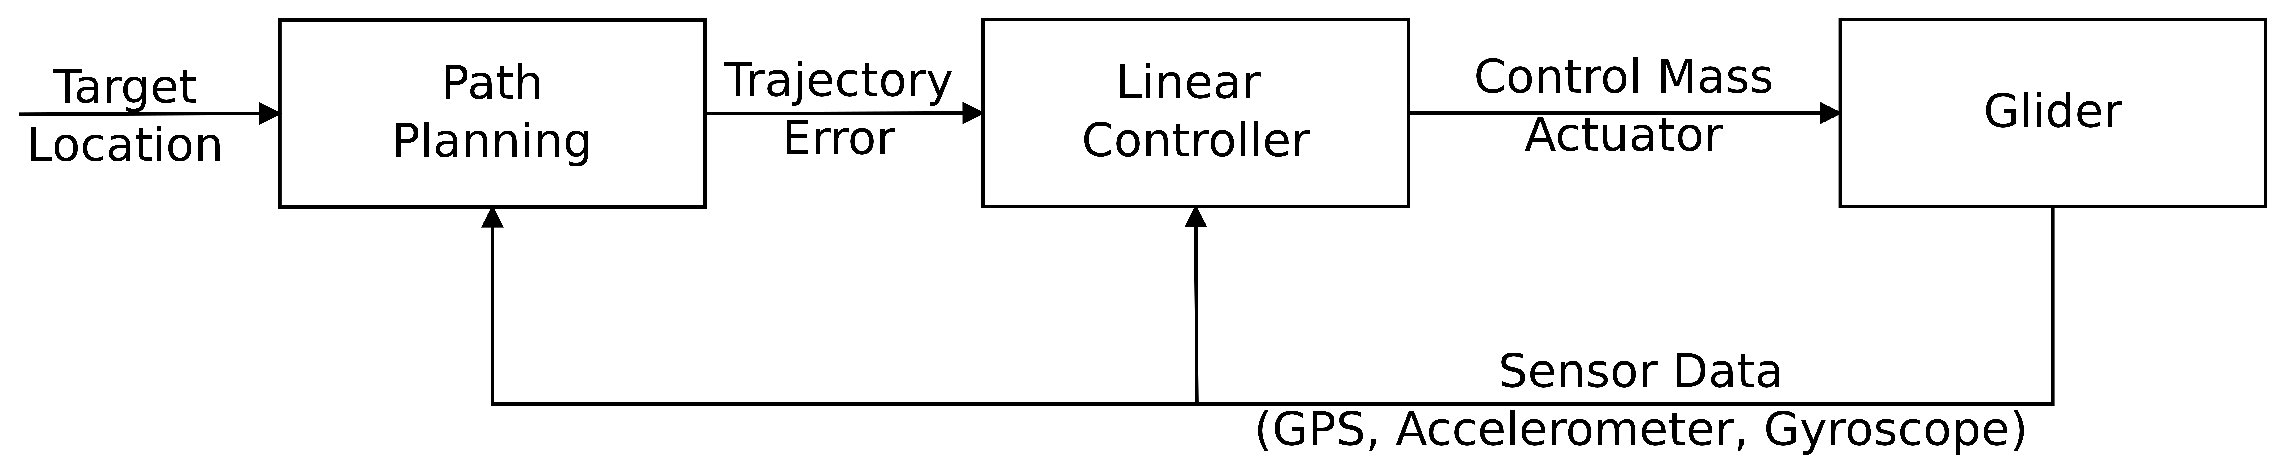
\includegraphics[width=0.8\columnwidth]{figs/flowchart}
    \caption{Top-Level Control Scheme}
    \label{fig:flowchart}
\end{figure}

The outer-loop block consists of a non-linear controller, instead of the typical
LTI setup.  The reasoning behind this choice was that, depending on the current
state of the craft, differing control objectives become active.  In
certain situations, the path planner will prioritize stable, forward flight,
while in others, it will attempt to minimize heading error and steer the craft
towards the target.  For more details, see \nameref{sec:ppdesign}, below.

The inner-loop controller was designed around the linearization of craft
dynamics provided by \cite{spottiswoode}.  For the purposes of the simulation,
all state variables are directly measurable.  A physical implementation would
not share this property, and so an observer would have to be designed to
estimate state.  However, the Separation Principle assures us that the
controller design is independant of the observer design, so the controller
designed here can be augmented with an observer later if the prototype is
actually built.  In the meantime, limiting the design to stabilization and
heading tracking simplifies the design.

\subsection{Performance Requirements}
\label{sec:perfreq}

Several considerations compete when establishing performance requirements for
the control system.  The craft must stay near the linearization point for the
model to remain accurate.  The control signal must remain within regions of
physical operation; since it corresponds to spherical coordinates of the control
mass, the horizontal plane serves as an extreme limit for absolute displacements
(in other words, the angular positions of the control mass are limited to at
most $\pm \pi/2$).  Therefore, the need for responses fast enough to stabilize
the craft compete with the need to keep control signals small.

In order to establish roll response specifications for the controller, the
open-loop system (i.e., the glider with constant, zero control input) was
simulated with an initial roll of $15\degree$ and measurements were made to
determine how quickly the system diverged from the linearization point - in
particular, the time it took for the roll or yaw to exceed $\pm45\degree$.  As
the craft is inherently stable in pitch, the pitch rise time requirement was
much more lax, and not based on any necessary behaviour the craft ought to have.
Physical limits of craft behaviour were also specified.  The derived
specifications are summarized in Table~\ref{tab:specs}.

\newglossaryentry{ess}{type=symbol,name={\ensuremath{e_{ss}}},
description={steady-state error}}
\newglossaryentry{trp}{type=symbol,name={\ensuremath{t_{r,pitch}}},
description={pitch response 90\% rise time}}
\newglossaryentry{trr}{type=symbol,name={\ensuremath{t_{r,roll}}},
description={roll response 90\% rise time}}
\newglossaryentry{urm}{type=symbol,name={\ensuremath{u_{r,max}}},
description={bounds on lateral control signal}}
\newglossaryentry{upm}{type=symbol,name={\ensuremath{u_{p,max}}},
description={bounds on longitudinal control signal}}

% Should we move performance requirements to Results? No; cf. grading sheet.
% '- The performance requirements belong here, in Methodology.
\begin{table}[b]
    \centering
    \begin{tabular}{|l|r|}
        \hline
        Performance metric & Value \\ \hline
        Steady-state error (\gls{ess}) & 0\degree \\
        Rise time, pitch (\gls{trp}) & 100 s \\
        Rise time, roll (\gls{trr}) & 3.0 s \\
        Lateral control signal bounds (\gls{urm}) & $\pm90\degree$ \\
        Longitudinal control signal bounds (\gls{upm}) & $\pm90\degree$ \\
        \hline
    \end{tabular}
    \caption{Performance specifications}
    \label{tab:specs}
\end{table}

\subsection{Path Planner Design}
\label{sec:ppdesign}
The outer-loop controller must handle the non-linearity of rotations within 3
dimensions and balance multiple objectives. Linear control schemes are
unsuitable to this variety of problem. Instead of a linear control scheme, a
modified gradient-descent minimization is run on an objective function that is
defined piecewise by the state of the craft. The priorities of this system are:
first, to reduce pitch if it exceeds $45^{\circ}$ from horizontal; second,
to reduce angles of attack and sideslip if their combined magnitude exceeds
$45^{\circ}$; and lastly, to minimize the difference between the craft's current
heading and the direction to the objective.

To avoid destabilizing the craft, the offset of the target heading to the
current heading is limited by running only a single step of this gradient
minimization in stead of running to completion. While this does not find the
optimal desired orientation immediatly, the craft's convergence on the target
heading will act to cause the target to converge towards the local minimum.

\subsection{Linear Quadratic Regulation}
\label{sec:lqr}
\newglossaryentry{Q}{type=symbol,name={\ensuremath{Q}},
description={LQR state penalty matrix}}
\newglossaryentry{R}{type=symbol,name={\ensuremath{R}},
description={LQR control signal penalty matrix}}
\newglossaryentry{K}{type=symbol,name={\ensuremath{K}},
description={controller feedback gain matrix}}

The control design methodology used for the inner-loop controller was that of
linear quadratic regulation.  In order to achieve perfect steady-state step
tracking, the system state was augmented with integrals of the output error (see
(\ref{eqn:z}), (\ref{eqn:xaug})).  No additional design complexity is required
for perfect steady-state step tracking.  Linear feedback (see
(\ref{eqn:ctrllaw})) is designed to optimize a quadratic cost function (see
(\ref{eqn:cost})).  The design parameters $\gls{Q}$ and $\gls{R}$ are chosen and
iteratively refined in order to meet the performance requirements.  The final
values for $\gls{Q}$, $\gls{R}$, and $\gls{K}$ are given in
Chapter~\ref{sec:results}.

\newglossaryentry{x}{type=symbol,name={\ensuremath{x}},
description={state vector}}
\newglossaryentry{xaug}{type=symbol,name={\ensuremath{\tilde{x}}},
description={state vector, augmented with \gls{z}}}
\newglossaryentry{z}{type=symbol,name={\ensuremath{z}},
description={integrated output error signal}}
\newglossaryentry{r}{type=symbol,name={\ensuremath{r}},
description={reference vector for system output}}
\newglossaryentry{y}{type=symbol,name={\ensuremath{y}},
description={system output signal}}
\newglossaryentry{u}{type=symbol,name={\ensuremath{u}},
description={control signal}}
\newglossaryentry{Kstate}{type=symbol,name={\ensuremath{K_{state}}},
description={portion of \gls{K} corresponding to state feedback}}
\newglossaryentry{Kref}{type=symbol,name={\ensuremath{K_{ref}}},
description={portion of \gls{K} corresponding to integral error feedback}}
\newglossaryentry{objfn}{type=symbol,name={\ensuremath{J(u)}},
description={LQR objective function}}

\begin{equation}
    \gls{z} = \int\limits_0^t \gls{r}(t) - \gls{y}(t) \; \textrm{d}t
    \label{eqn:z}
\end{equation}

\begin{equation}
    \gls{xaug} =
    \begin{pmatrix}
        \gls{x} \\ \gls{z}
    \end{pmatrix}
    \label{eqn:xaug}
\end{equation}

\begin{equation}
    \gls{u}
    =
    -
    \begin{pmatrix}
        \gls{Kstate} & \gls{Kref}
    \end{pmatrix}
    \gls{xaug}
    = - \gls{K} \gls{xaug}
    \label{eqn:ctrllaw}
\end{equation}

\begin{equation}
    \gls{objfn} = \int\limits_0^\infty \gls{xaug}^T(t)Q\gls{xaug}(t) +
    \gls{u}^T(t)R\gls{u}(t) \; \textrm{d}t
    \label{eqn:cost}
\end{equation}

\section{Simulation}
\label{sec:simulation}
In order to implement a simulation of the craft dynamics derived in
Section~\ref{sec:modelling}, a numerical approach was used.  Initial results
using a nested 4th/5th order Runge-Kutta method\footnote{Implemented using
MATLAB's \texttt{ode45}.} were numerically unstable.  Since there are non-linear
components in the system, notably the path planner, the behaviour of the system
will change more rapidly in some states than in others.  This can cause the
integration error in the RK solution to increase rapidly, forcing extremely
small step sizes.  Due to practical considerations, a faster simulation was
desired.

A stiff solver\footnote{Implemented using MATLAB's \texttt{ode15s}.} was used to
improve simulation runtimes.  The solver uses nested 1st/5th order techniques
implemented using the implicit method of backward differences, allowing much
greater timesteps \cite{SR97}.  Furthermore, the solver uses strategies to
minimize the frequency with which estimates of the problem's Jacobian matrix
must be calculated, further accelerating solution runtimes.

\chapter{Results and Discussion}
\label{sec:results}
% Final results must be presented based on your design or testing of your
% design.  Results should indicate the efficacy of your design efforts with
% respect to the objectives.

\section{Simulation Results}
\label{sec:simresults}
As the purpose of modelling was to obtain mathematical descriptions of the craft
behaviour, and no physical craft was obtained, the validity of the model was not
able to be tested with experimental data.  However, the implementation of the
model as a numerical simulation demonstrated physically reasonable behaviour;
running the simulation with different initial conditions (ICs) showed,
variously, long-term pitch stability (see Fig.~\ref{fig:pitchstability}), roll
and yaw instability due to nonzero ICs (see Fig.~\ref{fig:rollinstability}), and
other reasonable results, such as the conservation of energy (in
Fig.~\ref{fig:pitchstability}, once terminal velocity has been reached, energy
steadily decreases due to drag effects).

\begin{figure}
    \begin{center}
        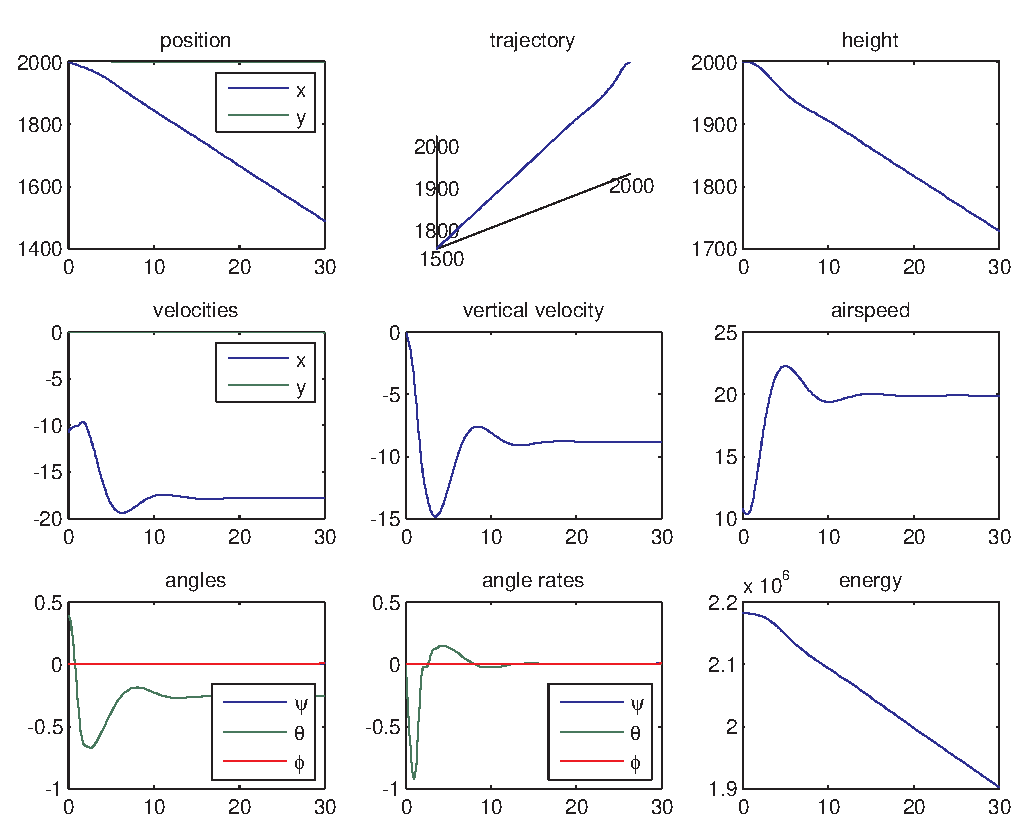
\includegraphics[width=0.8\columnwidth]{figs/pitchstable}
    \end{center}
    \caption{Simulation demonstrating long-term open-loop pitch stability.}
    \label{fig:pitchstability}
\end{figure}

\begin{figure}
    \begin{center}
        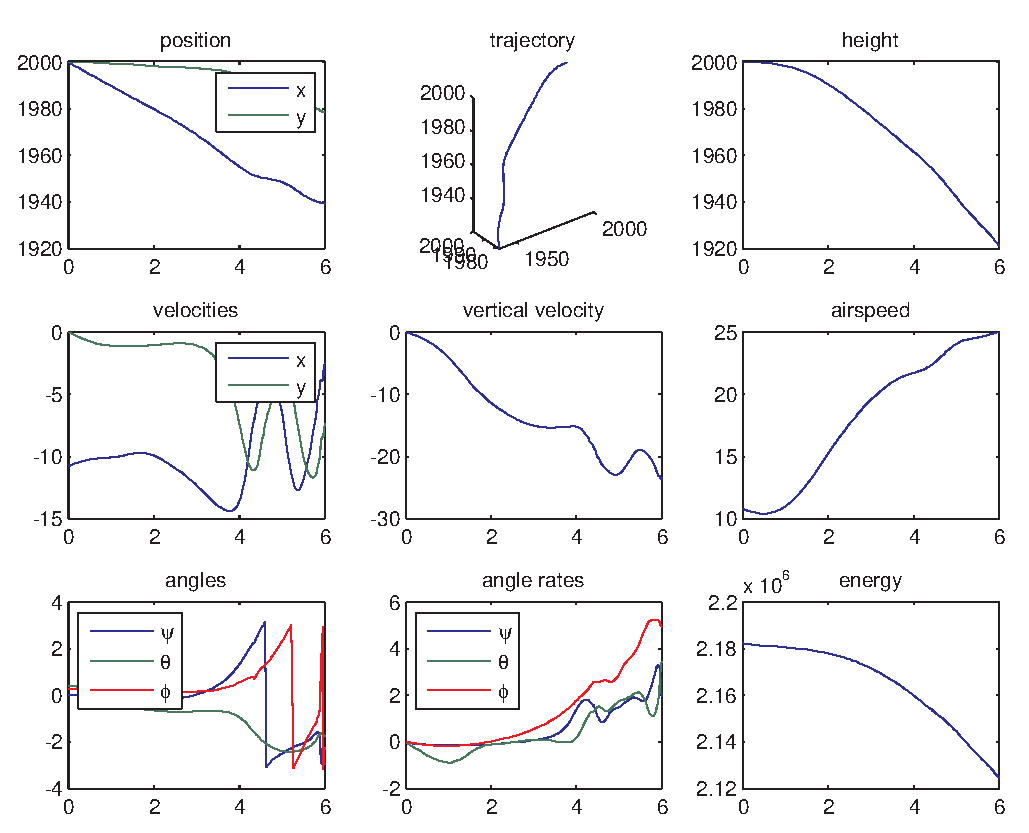
\includegraphics[width=0.8\columnwidth]{figs/rollunstable}
    \end{center}
    \caption{Simulation demonstrating open-loop roll and yaw instability.}
    \label{fig:rollinstability}
\end{figure}

\subsection{Controller Implementation}
\label{sec:ctrlimpl}
The linearized model presented in \cite{spottiswoode} uses disturbance
parameters for the yaw, pitch, and roll attitudes.  The reference angles for
these disturbance parameters are their steady-state values; however, these
steady-state values of craft parameters may be computationally
intensive to obtain for arbitrary flight configurations, and in fact may not
exist, for example when the craft is in a roll.
This prevents the calculation of appropriate disturbance values to
pass to the control logic during simulation.  The result of these difficulties
is that the controller designed using the methodology outlined in
Section~\ref{sec:ctrldes} cannot be fully implemented without making significant
changes to the model from \cite{spottiswoode}.

\section{Controller Design}

\newglossaryentry{ctrb}{type=symbol,name={\ensuremath{\mathcal{C}}},
description={standard controllability matrix}}
\newglossaryentry{A}{type=symbol,name={\ensuremath{A}},
description={state matrix}}
\newglossaryentry{B}{type=symbol,name={\ensuremath{B}},
description={input matrix}}
\newglossaryentry{C}{type=symbol,name={\ensuremath{C}},
description={output matrix}}
\newglossaryentry{n}{type=symbol,name={\ensuremath{n}},
description={number of states in \gls{x}}}

The linearized model in \cite{spottiswoode} was initially found to be
uncontrollable when using the standard controllability matrix given in
(\ref{eqn:ctrb}).  Note that $\gls{n}$ is the number of states (i.e., $\gls{A}$
is $\gls{n} \times \gls{n}$).
\begin{equation}
    \gls{ctrb} = [\gls{B} \;\, \gls{A}\gls{B} \;\, \gls{A}^2\gls{B} \;\, \ldots
    \;\, \gls{A}^{\gls{n}-1}\gls{B}]
    \label{eqn:ctrb}
\end{equation}

As this controllability test involves taking high powers of the $\gls{A}$
matrix, it has poor numeric properties.  The condition number of $\gls{ctrb}$
was found to be over 7.5e17.  When calculating the condition number of
$\gls{ctrb}$ for the plant augmented with integral action, it was large enough
that MATLAB simply classified it as infinite.  As a result, $\gls{ctrb}$ was
found to be rank-deficient.

\newglossaryentry{eig}{type=symbol,name={\ensuremath{\lambda}},sort=lambda,
description={an eigenvalue of \gls{A}}}
\newglossaryentry{I}{type=symbol,name={\ensuremath{I}},
description={the identity matrix}}

To avoid these numeric issues, the PBH controllability test was used (see
(\ref{eqn:pbhctrb})).  By evaluating the controllability of each mode separately,
condition numbers are kept much smaller.  The largest condition number for any
of the matrices used was found to be approximately 469, and the system was shown
to be controllable (all of the matrices were full rank).
\begin{equation}
    \textrm{rank}([\gls{A} - \gls{eig} \gls{I} \;\, \gls{B}]) = \gls{n} \quad
    \forall \; \gls{eig} \in \textrm{eig}(\gls{A})
    \label{eqn:pbhctrb}
\end{equation}

Pole-zero maps of the linearized system were prepared to analyze for performance
limitations.  The plots can be found in Appendix~\ref{sec:ctrlplots}.

\section{Controller Performance}
Although the difficulties detailed in \nameref{sec:ctrlimpl}, above, prevented
measuring the designed controller's performance in the nonlinear simulation, it
was simulated using the linearized plant to measure performance and iterate
design choices for the LQR parameters $\gls{Q}$ and $\gls{R}$ (cf.
Section~\ref{sec:lqr}).  The final values are given in
Appendix~\ref{sec:ctrlvals}, and simulations demonstrating that the rise time
specifications given in Section~\ref{sec:perfreq} have been met are shown in
Fig.~\ref{fig:linrisetime}.

\begin{figure}
    \centering
    \subfloat[Pitch
    performance]{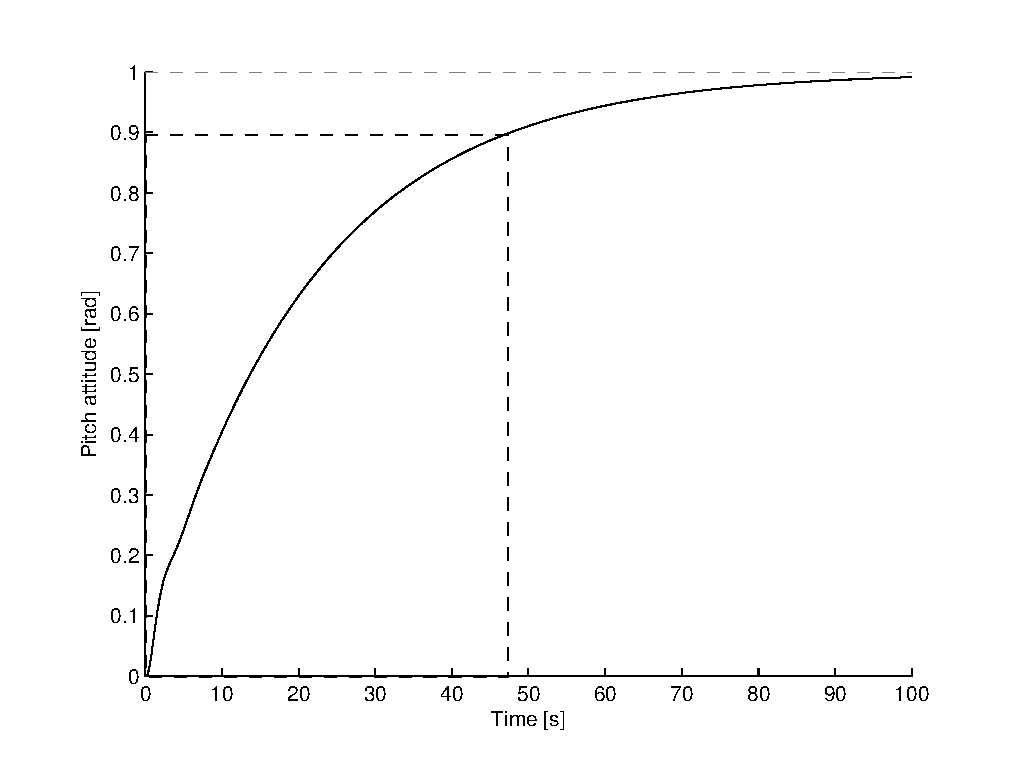
\includegraphics[width=0.8\columnwidth]{figs/pitchresp}} \\
    \subfloat[Roll
    performance]{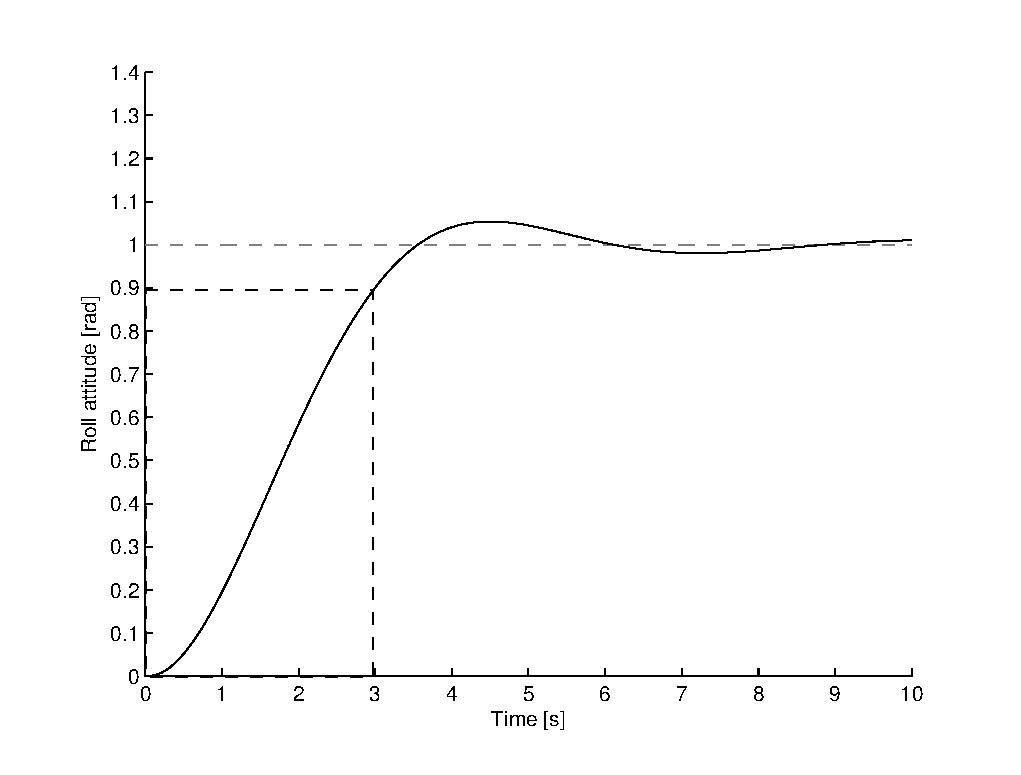
\includegraphics[width=0.8\columnwidth]{figs/rollresp}}
    \caption{Simulation of linear model showing rise-time performance.}
    \label{fig:linrisetime}
\end{figure}

\pagebreak

\section{Objectives}
Due to the difficulties mentioned in \nameref{sec:ctrlimpl}, above, the final
controller design was not able to be evaluated in the nonlinear simulation.  As
a result, it is unclear whether the controller as designed meets all of the
objectives given in Section~\ref{sec:objs}.  However, simulations of the
linearized model show that the controller met the performance requirements
established for it.  If these requirements were correctly chosen, then the
controller will stabilize the nonlinear system and aim the simulated craft
toward the destination.

However, lacking the plans for the WRT's glider, it was not possible to
determine acceptable bounds on the landing conditions. The alternate glider
parameters used did not contain sufficient detail to estimate these for that
craft either.  Due to this lack of information and timeline overruns elsewhere,
plans for accomodating landing requirements were scrapped.

\chapter{Conclusions}
% You must provide a clear, succinct account of your contributions to the design
% and solution of the identified problem.  Shortcomings should be identified
% (nothing is ever perfect!).  Future recommendations must be provided and can
% (if appropriate) be formulated as a basis for a future Systems Design
% workshop.
Due to external factors, as well as the ambitious nature of the project, some
contractions in scope were required.  As the actual glider to be built for the
WRT was not constructed and its plans were never delivered, a model for another
hang glider was substituted.  This model was derived using physical principles
and simulated using numerical methods (cf. Sections \ref{sec:modelling},
\ref{sec:simulation}).  Of the objectives given in Section \ref{sec:objs}, those
of flight stabilization and waypoint navigation were considered and designed
for.  As far as can be measured, these objectives appear to have been met; see
Chapter~\ref{sec:results} for more details.  Techniques for landing the craft
safely were not considered.

\section{Recommendations}
\label{sec:recommendations}
The greatest shortcomings of the design at the moment are the difficulties
described in Section~\ref{sec:simresults}, preventing the integration of the
controller in the nonlinear simulation.  If this can be overcome, then the
controller can be simulated in a fuller context and evaluated to determine
whether the objectives of the controller design have been met.

If the Waterloo Rocketry Team still desires an autonomous hang glider to deploy
from their rocket in a future competition, then craft plans must be provided to
replace the model from \cite{spottiswoode} with one corresponding to the actual
craft.  Experimental testing, potentially involving either a scale model in a
wind tunnel or a full model in free flight, should be used to refine the model.
With the improved and validated model in hand, the controller design presented
here should be re-evaluated to ensure that it meets the established performance
specifications.

The objective of landing the craft safely should be considered in a future
project.  With the groundwork laid by this project and the support of the WRT,
it should take one or two competent individuals approximately two to three
months to research and simulate different landing techniques.

Finally, with a validated model of the real-world craft, reiteration and
validation of the existing controller design and design methodology, and landing
techniques tested in simulation, the craft and controller can be validated with
free-flight testing.

\appendix

\chapter{Timeline}
% Provide a copy of your original timeline and a description of how well you met
% the objectives initially projected.  Provide an explanation for situations
% where the timeline requirements were not met.  This information is best placed
% in an Appendix.


Aggressive timeline, poor implementation decisions, and dependence on external
cooperation all contributed to the need for reduction in scope of the initial
plan.

At the outset of the project, the group was lacking the skills and insights,
particularly into dynamics and control theory. These were learned by group
members as required to complete their tasks. The plan did not account for the
time taken in learning and associated naive mistakes.

Several suboptimal decisions were made regarding implementation strategy. One
salient example is the failure to invest in a $3^{rd}$ party physics simulation
system. These decisions led to much additional work, such as debugging a
home-grown physics simulation system, only tangential to the objectives.

The project was initially framed in the context of the UW Rocketry Team's needs.
However, the glider's mechanical design has yet to be made available to the team or
this project. Additionally, both engine tests run by the team to date have
resulted in destructive failures. Lacking parameters for the glider, a prototype
of the glider, engine force and noise characteristics, or a rocket to use in
test flights; many of the scheduled activities cannot be accomplished.

The initial timeline, as well as its current state of completion, is summarized
below.

\begin{longtable} { c p{2.5in}@{ } c c c } 
    \hline
    Month & Task & Status & Andrew & Peter \\
    \hline
    Sep
        & Identify task & Completed & \checkmark & \checkmark \\
        & Identify important unknowns & Completed & \checkmark & \checkmark \\
        & Research wing dynamics & Completed & \checkmark & \checkmark \\
        & Obtain prior art & Completed & \checkmark & \\
    \hline
    Oct
        & Design Plan & Completed & \checkmark \\
        & Glider component breakdown & Completed & \checkmark & \\
        & Glider team PDR & Completed & \checkmark & \checkmark \\
        & Glider stable flight model & Completed & & \checkmark \\
        & Actuator and sensor selection & Abandoned & \checkmark & \\
    \hline
    Nov
        & Actuator and sensor parts acquisition & Abandoned & \checkmark & \\
        & Glider deployment strategy & Adopted by WRT & & \checkmark \\
        & Actuator and sensor testing & Abandoned & \checkmark & \\
        & Steady flight controller design & Partially Completed & \checkmark & \\
    \hline
    Dec
        & Glider mechanical design completed and presented (external) & Not Done & & \\
        & Website Summary & Completed & & \checkmark \\
        & Interim Progress Report & Completed & \checkmark & \\
    \hline
    Jan
        & WRT engine tests (external) & Failed & & \\
        & Steady flight controller design (continued) & Partially Completed & \checkmark & \\
        & Adjustment/augmentation of & Adopted by WRT & \checkmark & \\
            & controller for deployment task  \\
        & Rocket flight vibration modeling & Abandoned & & \checkmark \\
    \hline
    Feb
        & WRT test flight (external) & Postponed & & \\
        & Controller parts acquisition & Abandoned & \checkmark & \\
        & Rocket flight shock/forces modeling & Abandoned & & \checkmark \\
    \hline
    Mar
        & Assembly & Abandoned & \checkmark & \checkmark \\
        & Glider test flight & Abandoned & \checkmark & \checkmark \\
        & 2 week buffer & & & \\
    \hline
    Apr
        & Final Report & Ongoing & \checkmark & \checkmark \\
        & Conference Summary & Ongoing & \checkmark & \checkmark \\
        & Project Video & Ongoing & \checkmark & \checkmark \\
        & Symposium Presentation Materials & Completed & \checkmark & \checkmark \\
        & Symposium & Completed & \checkmark & \checkmark \\
    \hline
    Jun
        & Intercollegiate Rocket \\
            & Engineering Competition & & \checkmark & \checkmark \\
    \hline
\end{longtable}

\chapter{Control Analysis Plots}
\label{sec:ctrlplots}
Plots demonstrating pole-zero maps for the linearized plant follow.
Figures~\ref{fig:long1} through \ref{fig:long4} show plots for transfer
functions starting with the longitudinal control input, while
Figures~\ref{fig:lat1} through \ref{fig:lat5} show those for transfer functions
beginning with the lateral control input.

\begin{figure}[h]
    \centering
    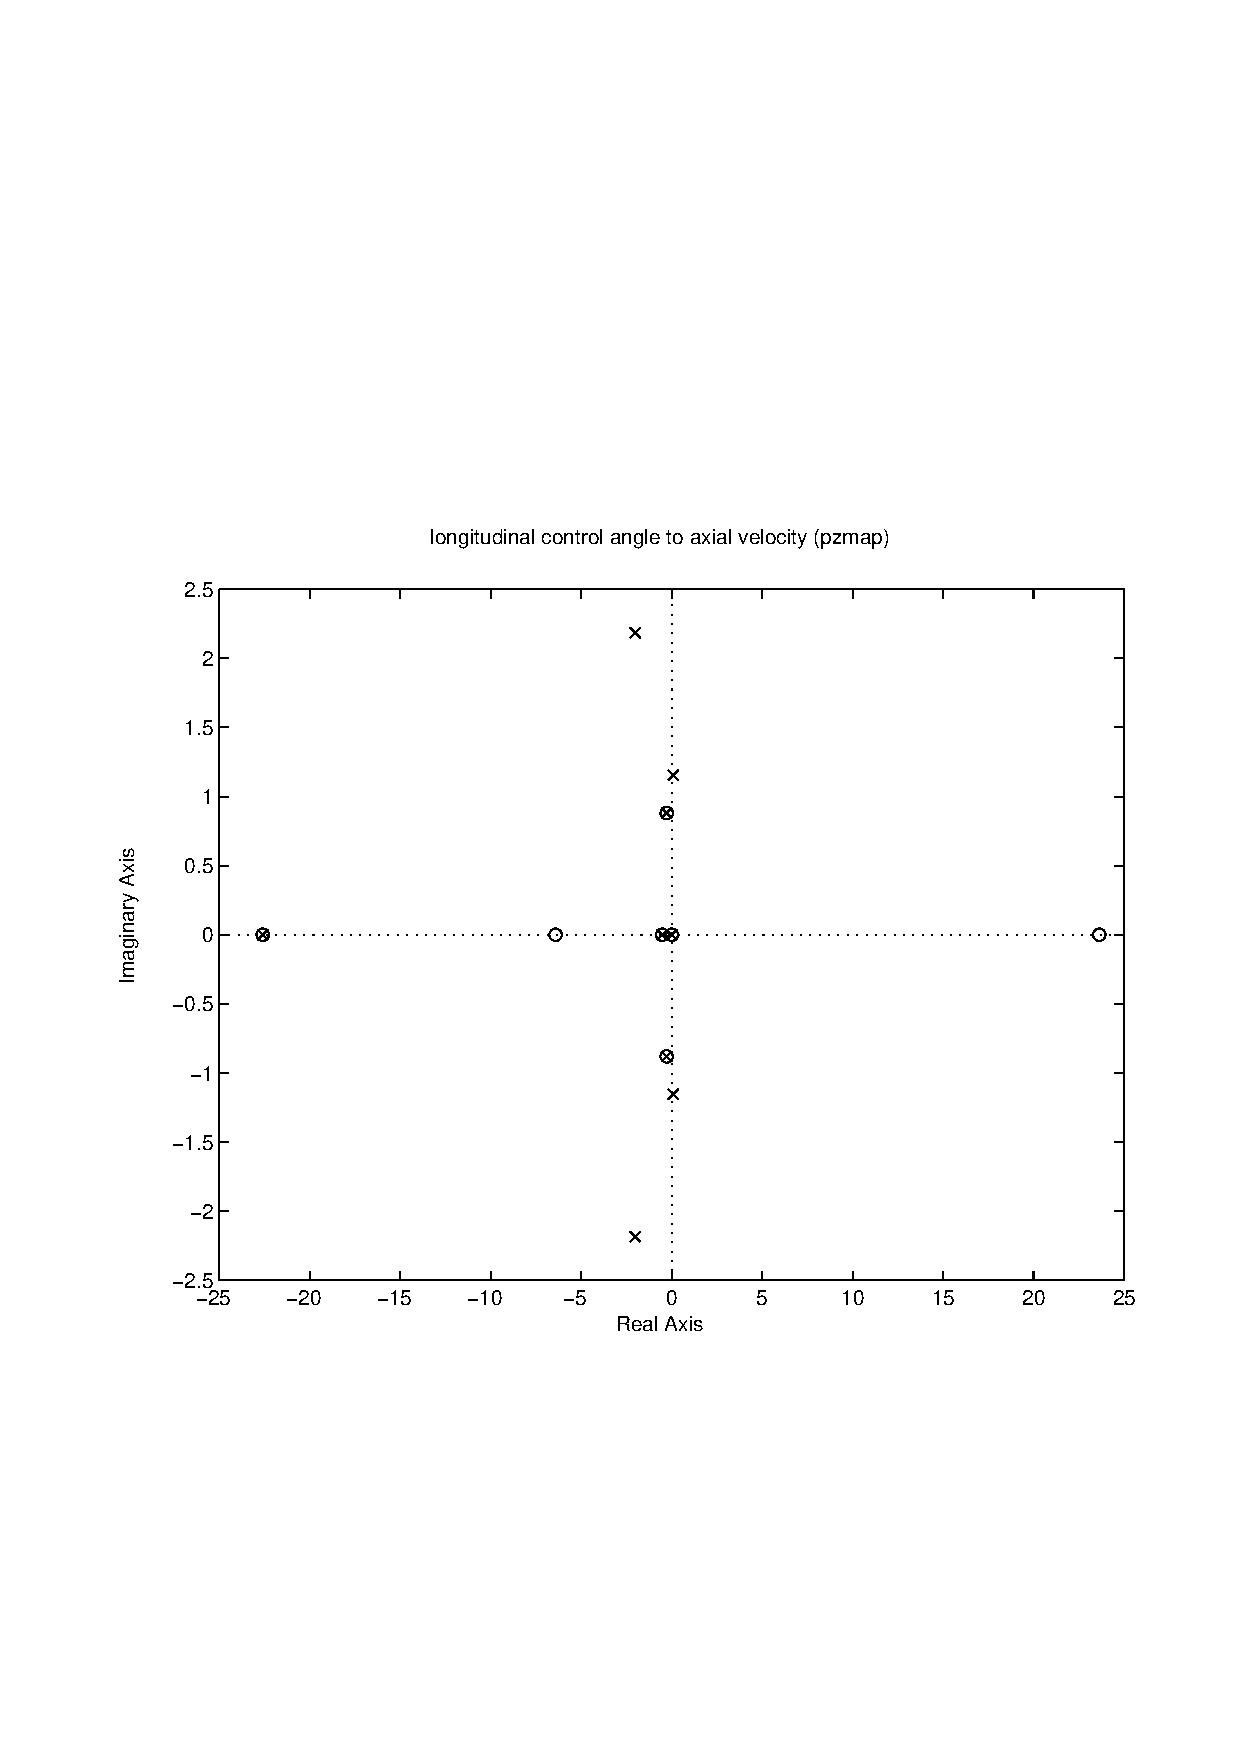
\includegraphics[width=0.8\columnwidth]{figs/11pz}
    %\caption{Pole-zero plots for transfer functions originating with
    %longitudinal control input.}
    \caption{Axial velocity}
    \label{fig:long1}
\end{figure}

\begin{figure}[h]
    \centering
    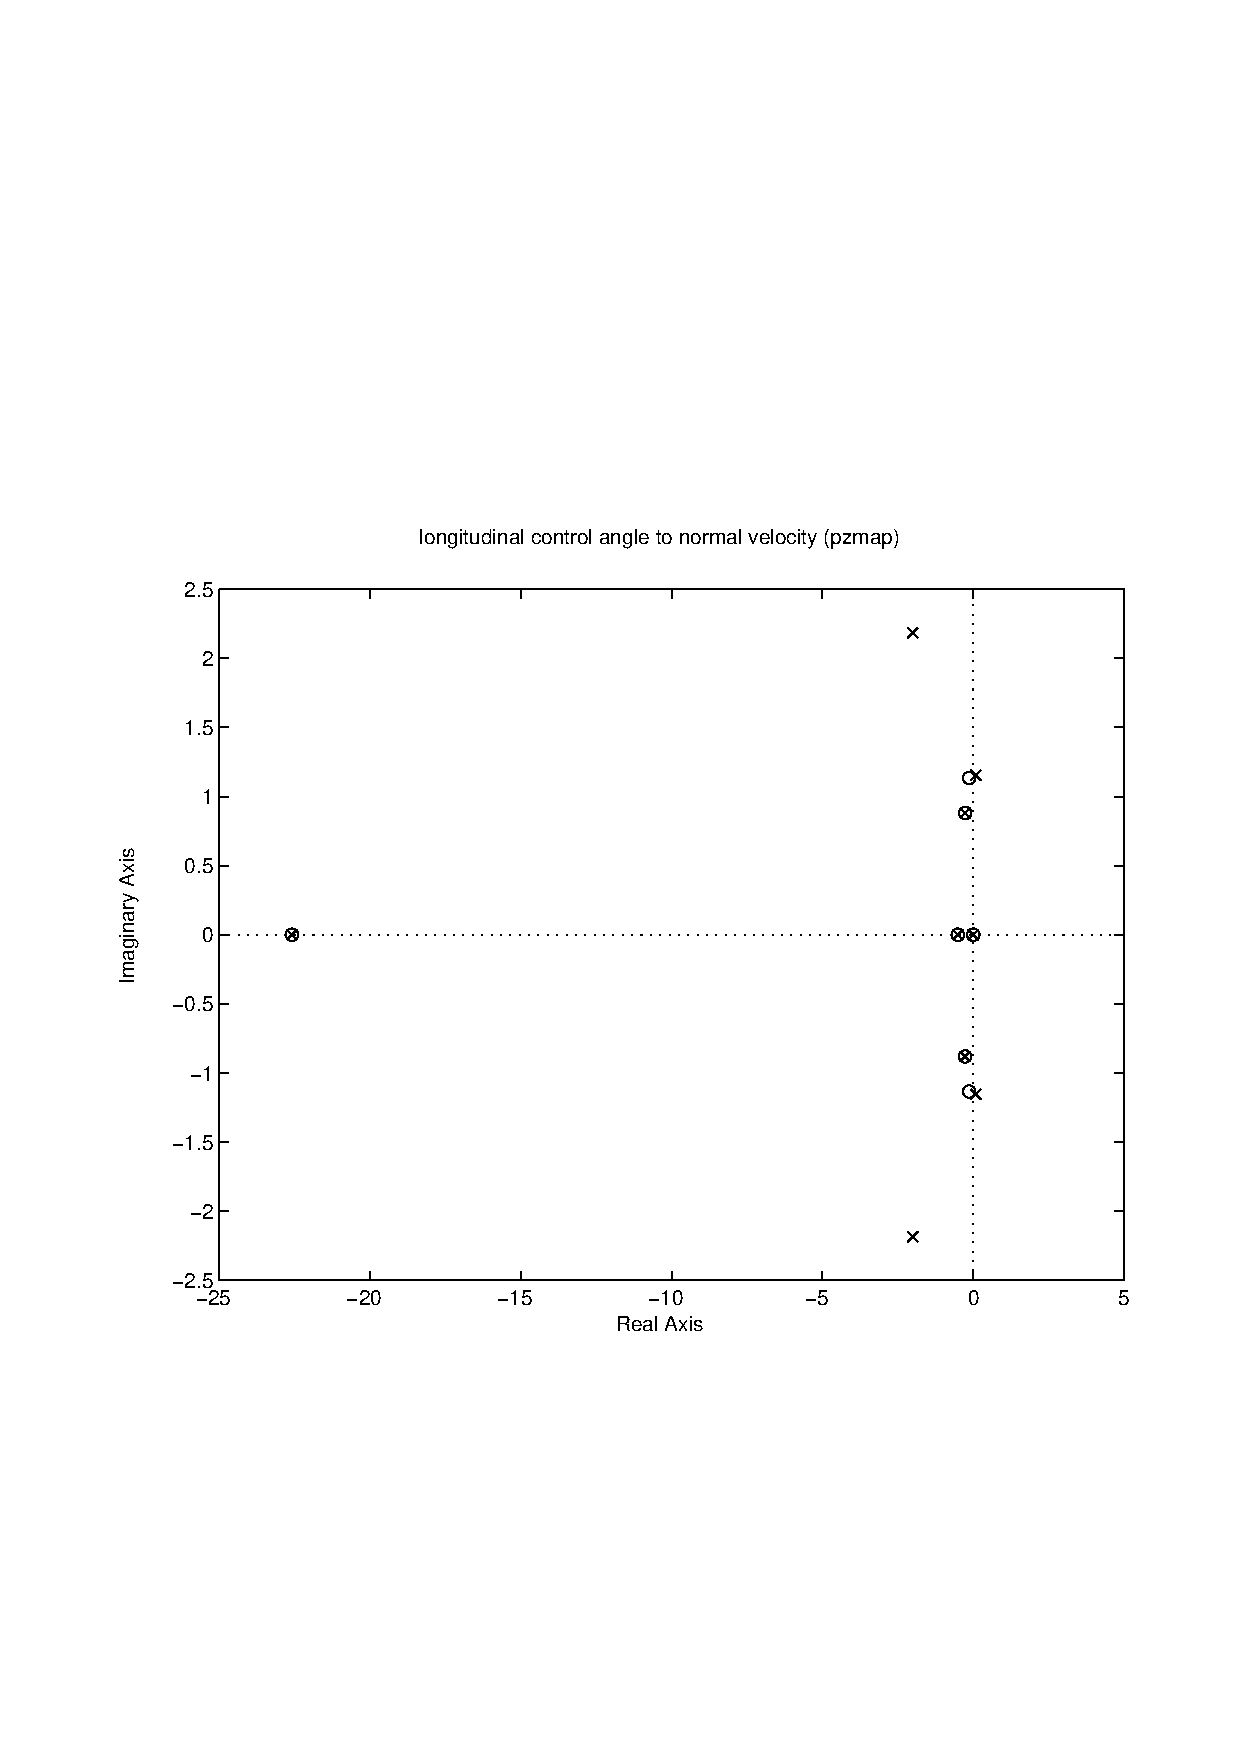
\includegraphics[width=0.8\columnwidth]{figs/12pz}
    \caption{Normal velocity}
\end{figure}

\begin{figure}[h]
    \centering
    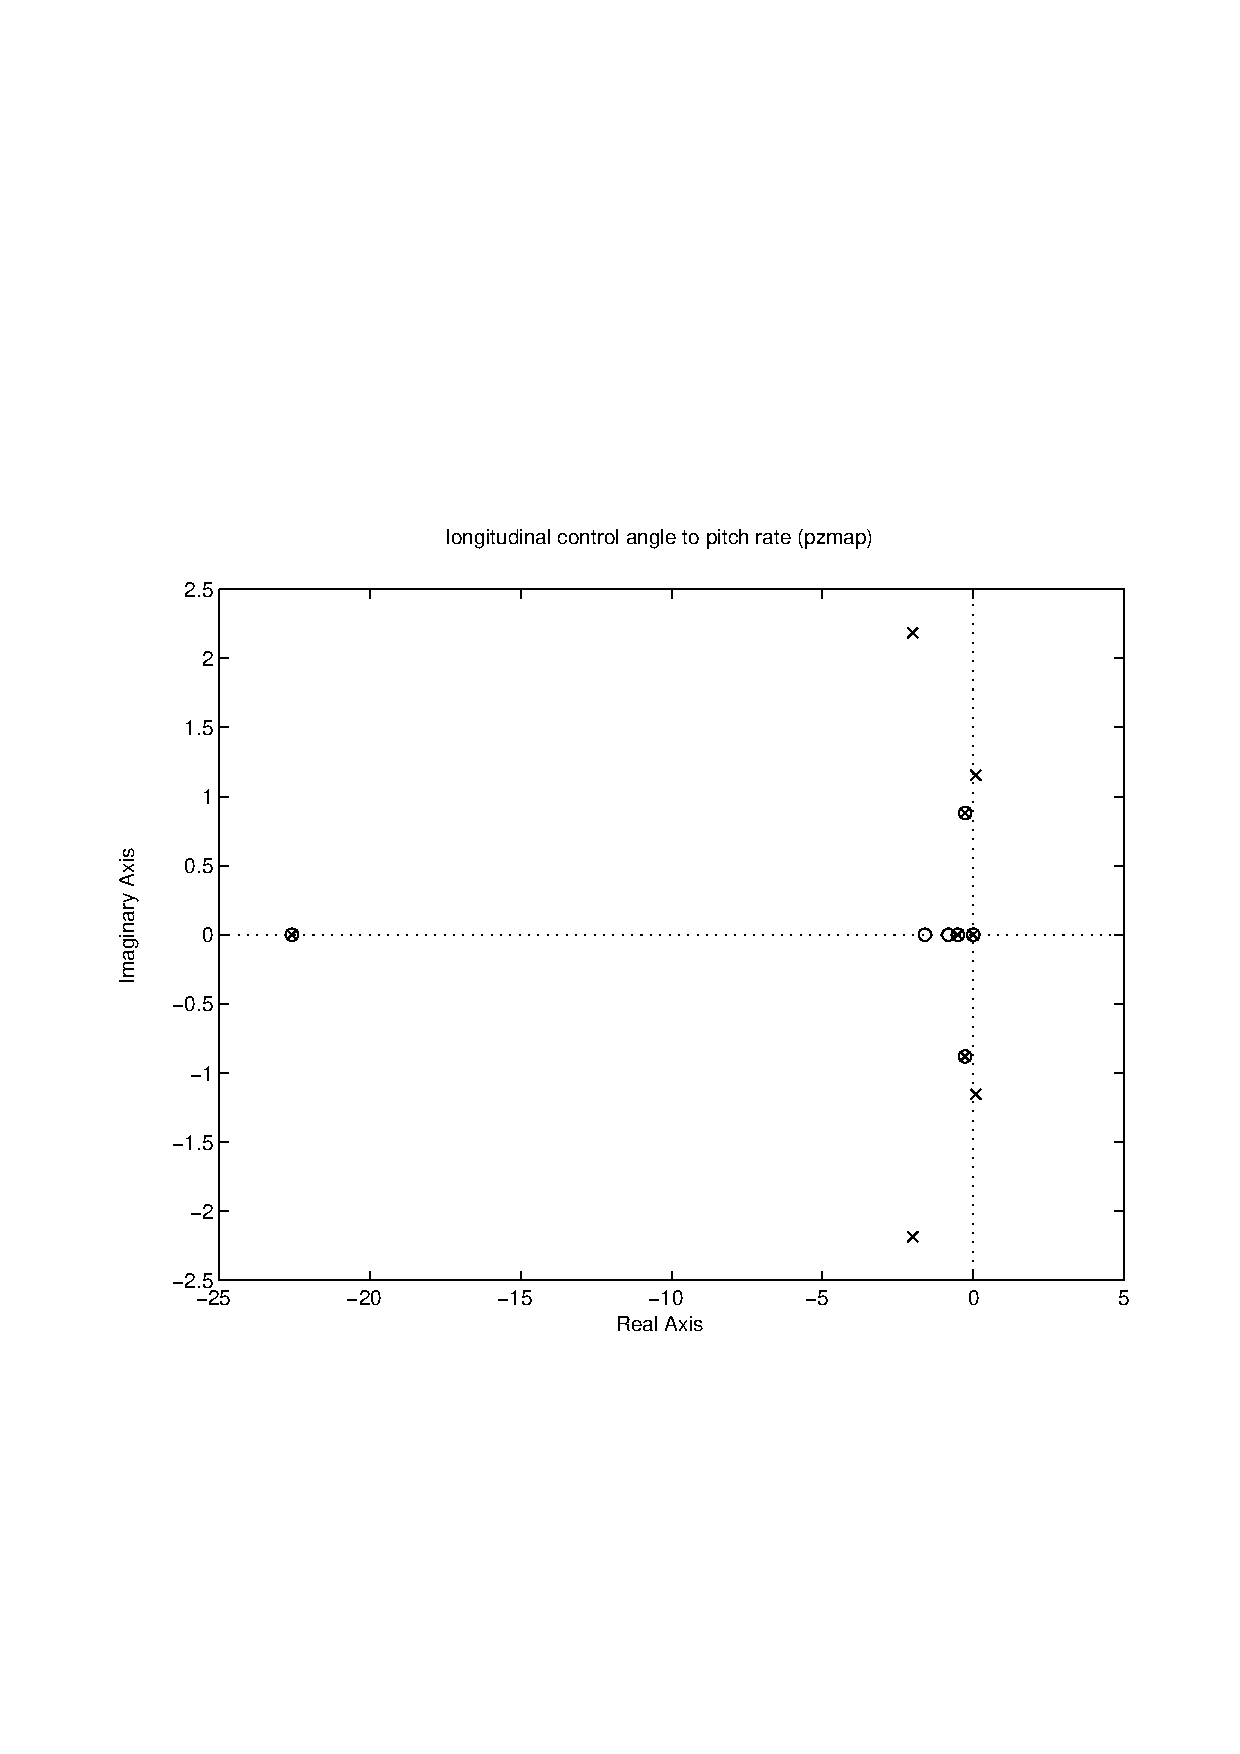
\includegraphics[width=0.8\columnwidth]{figs/13pz}
    \caption{Pitch rate}
\end{figure}

\begin{figure}[h]
    \centering
    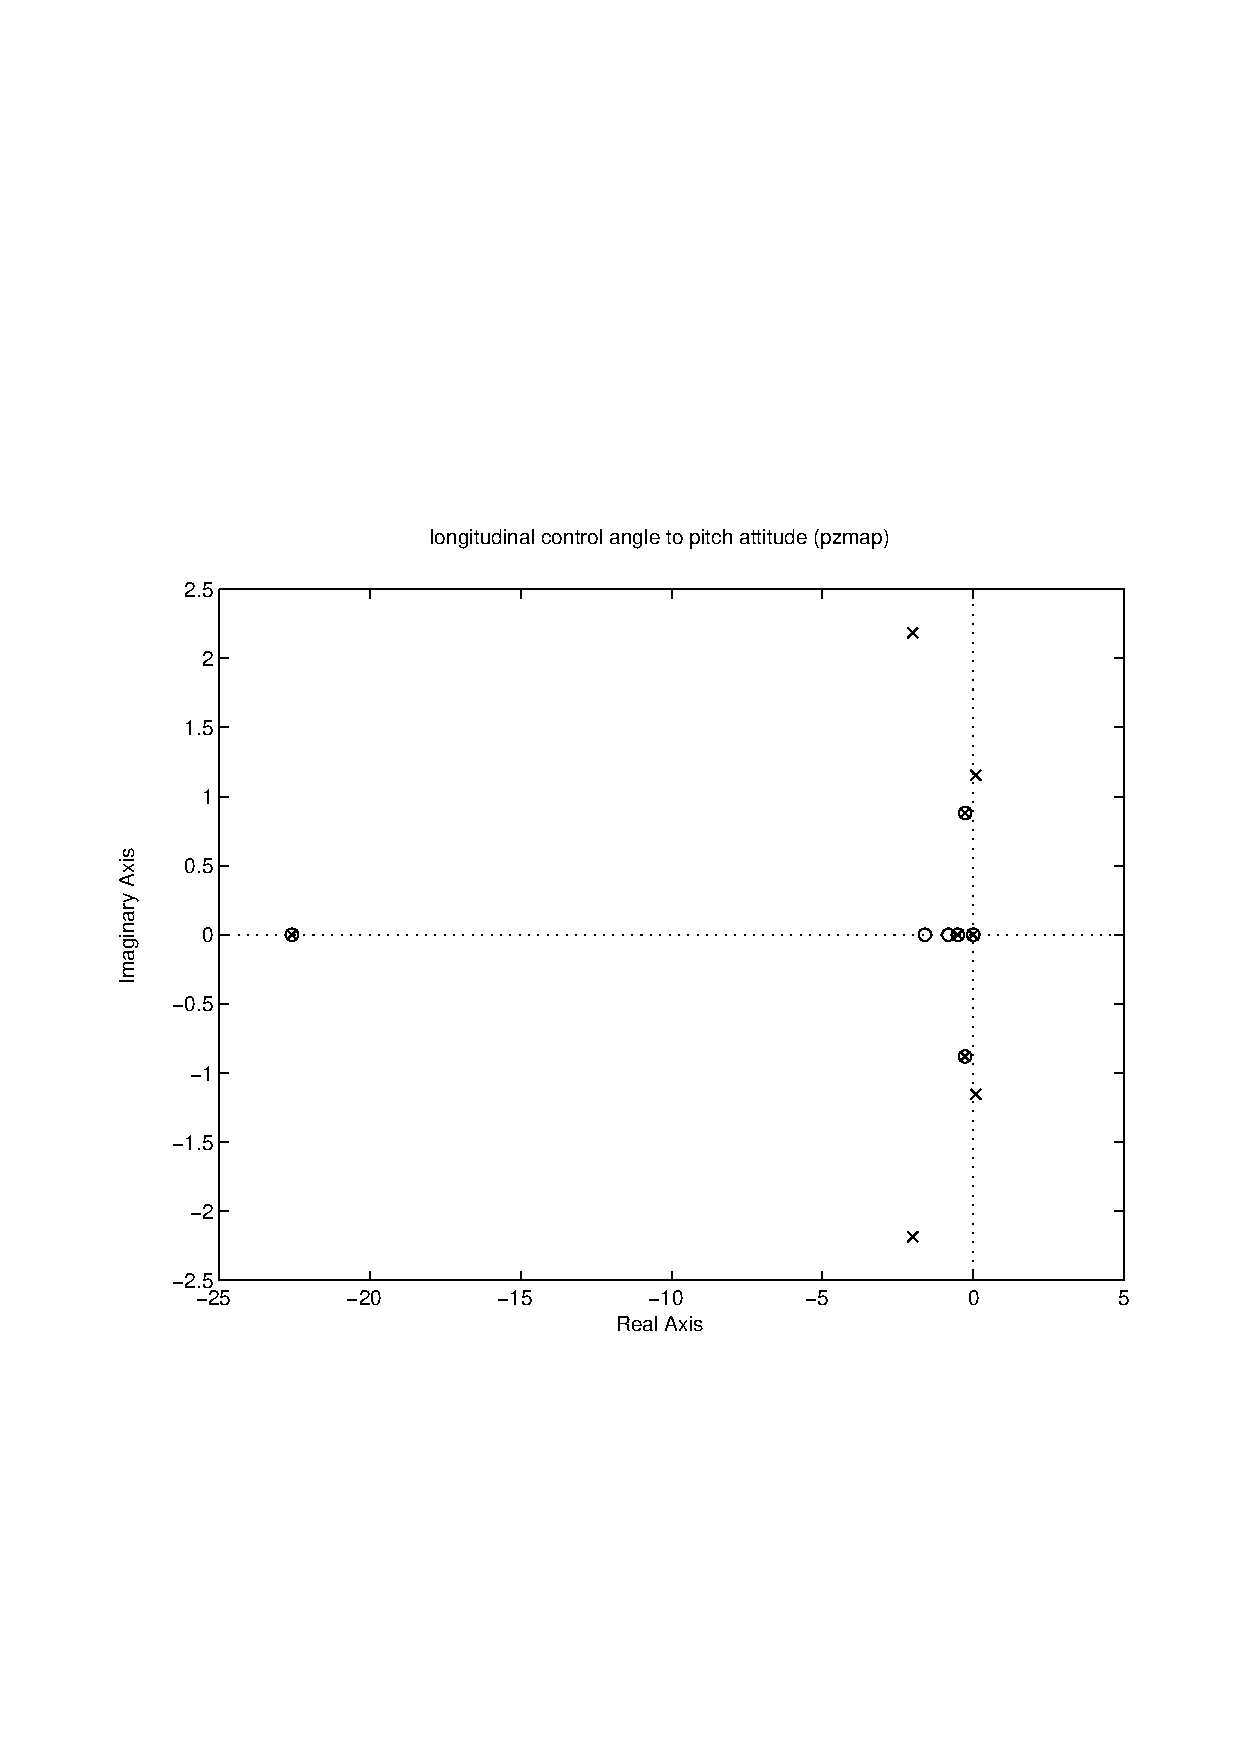
\includegraphics[width=0.8\columnwidth]{figs/14pz}
    \caption{Pitch attitude}
    \label{fig:long4}
\end{figure}

\begin{figure}[h]
    \centering
    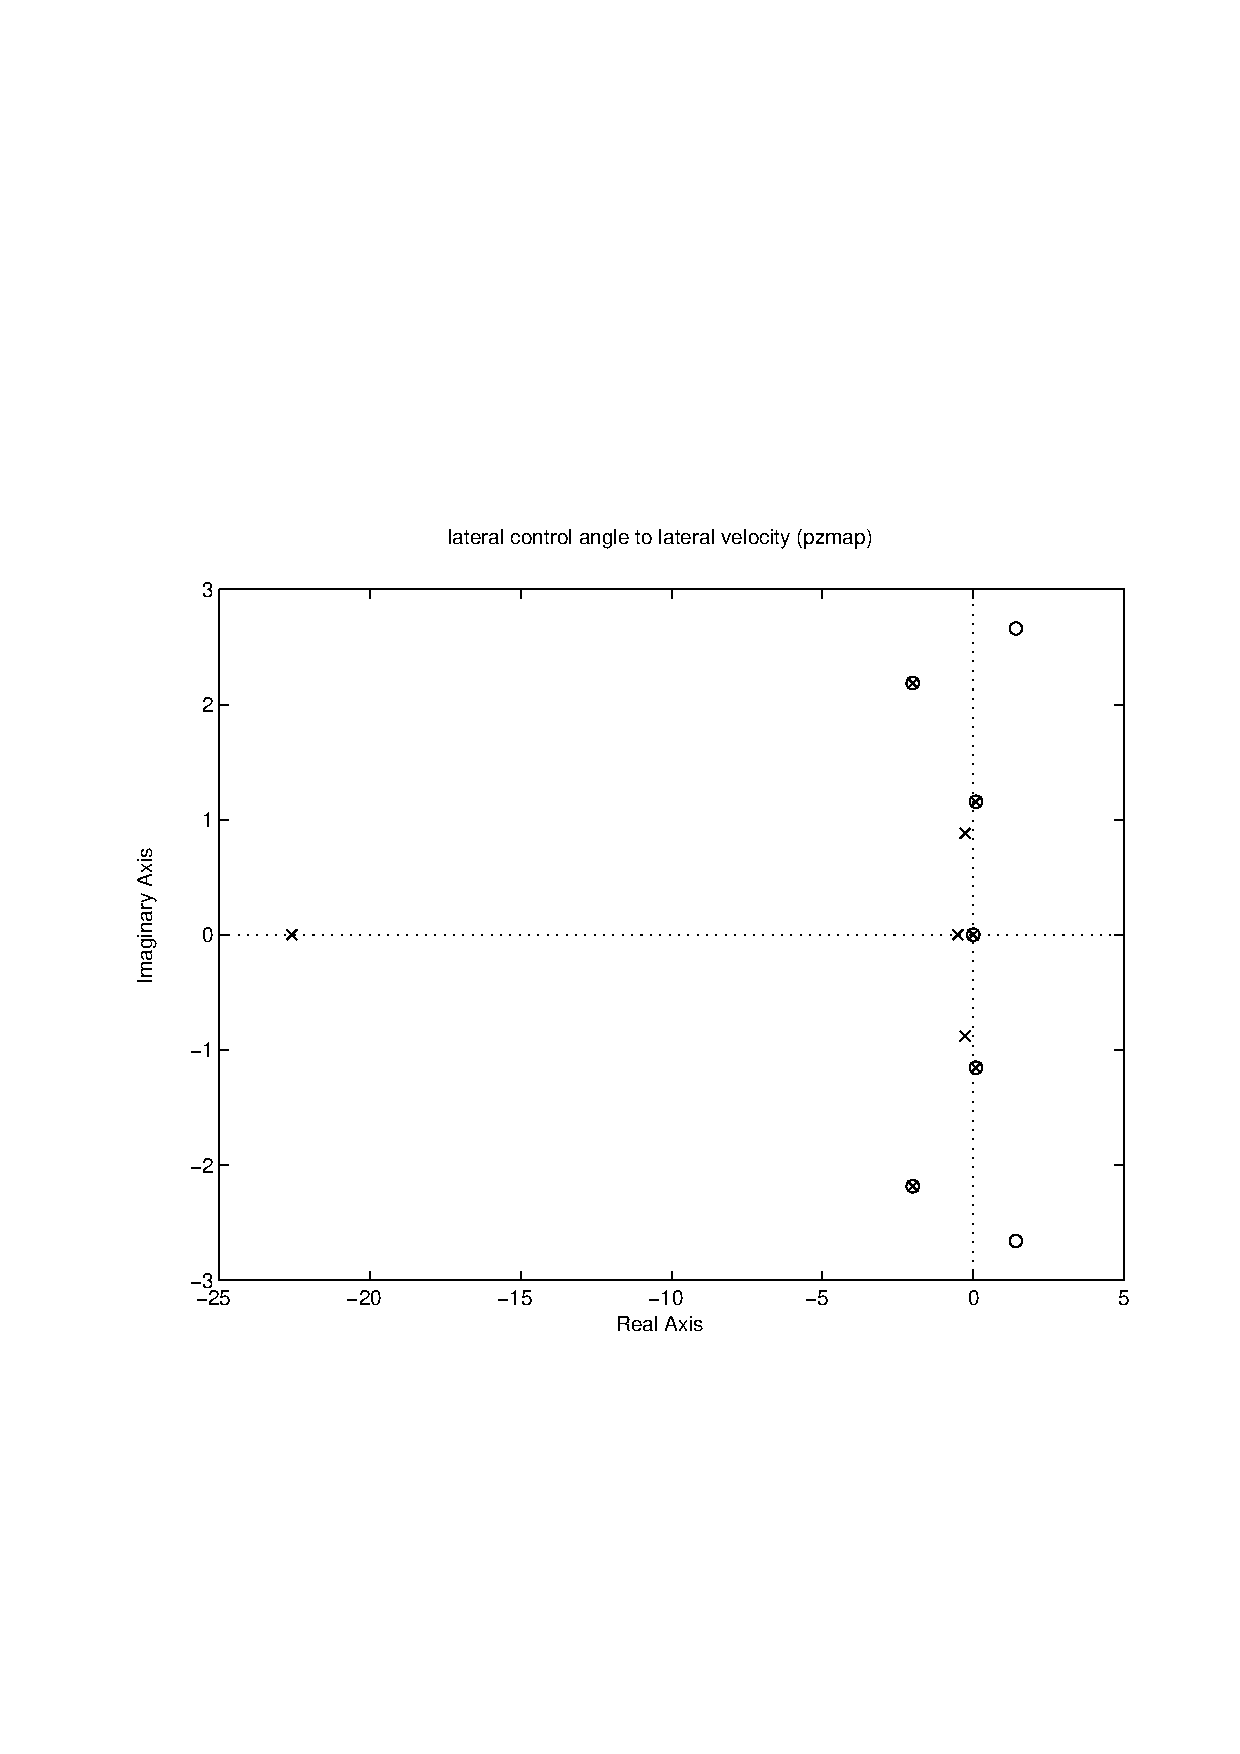
\includegraphics[width=0.8\columnwidth]{figs/25pz}
    \caption{Lateral velocity}
    \label{fig:lat1}
\end{figure}

\begin{figure}[h]
    \centering
    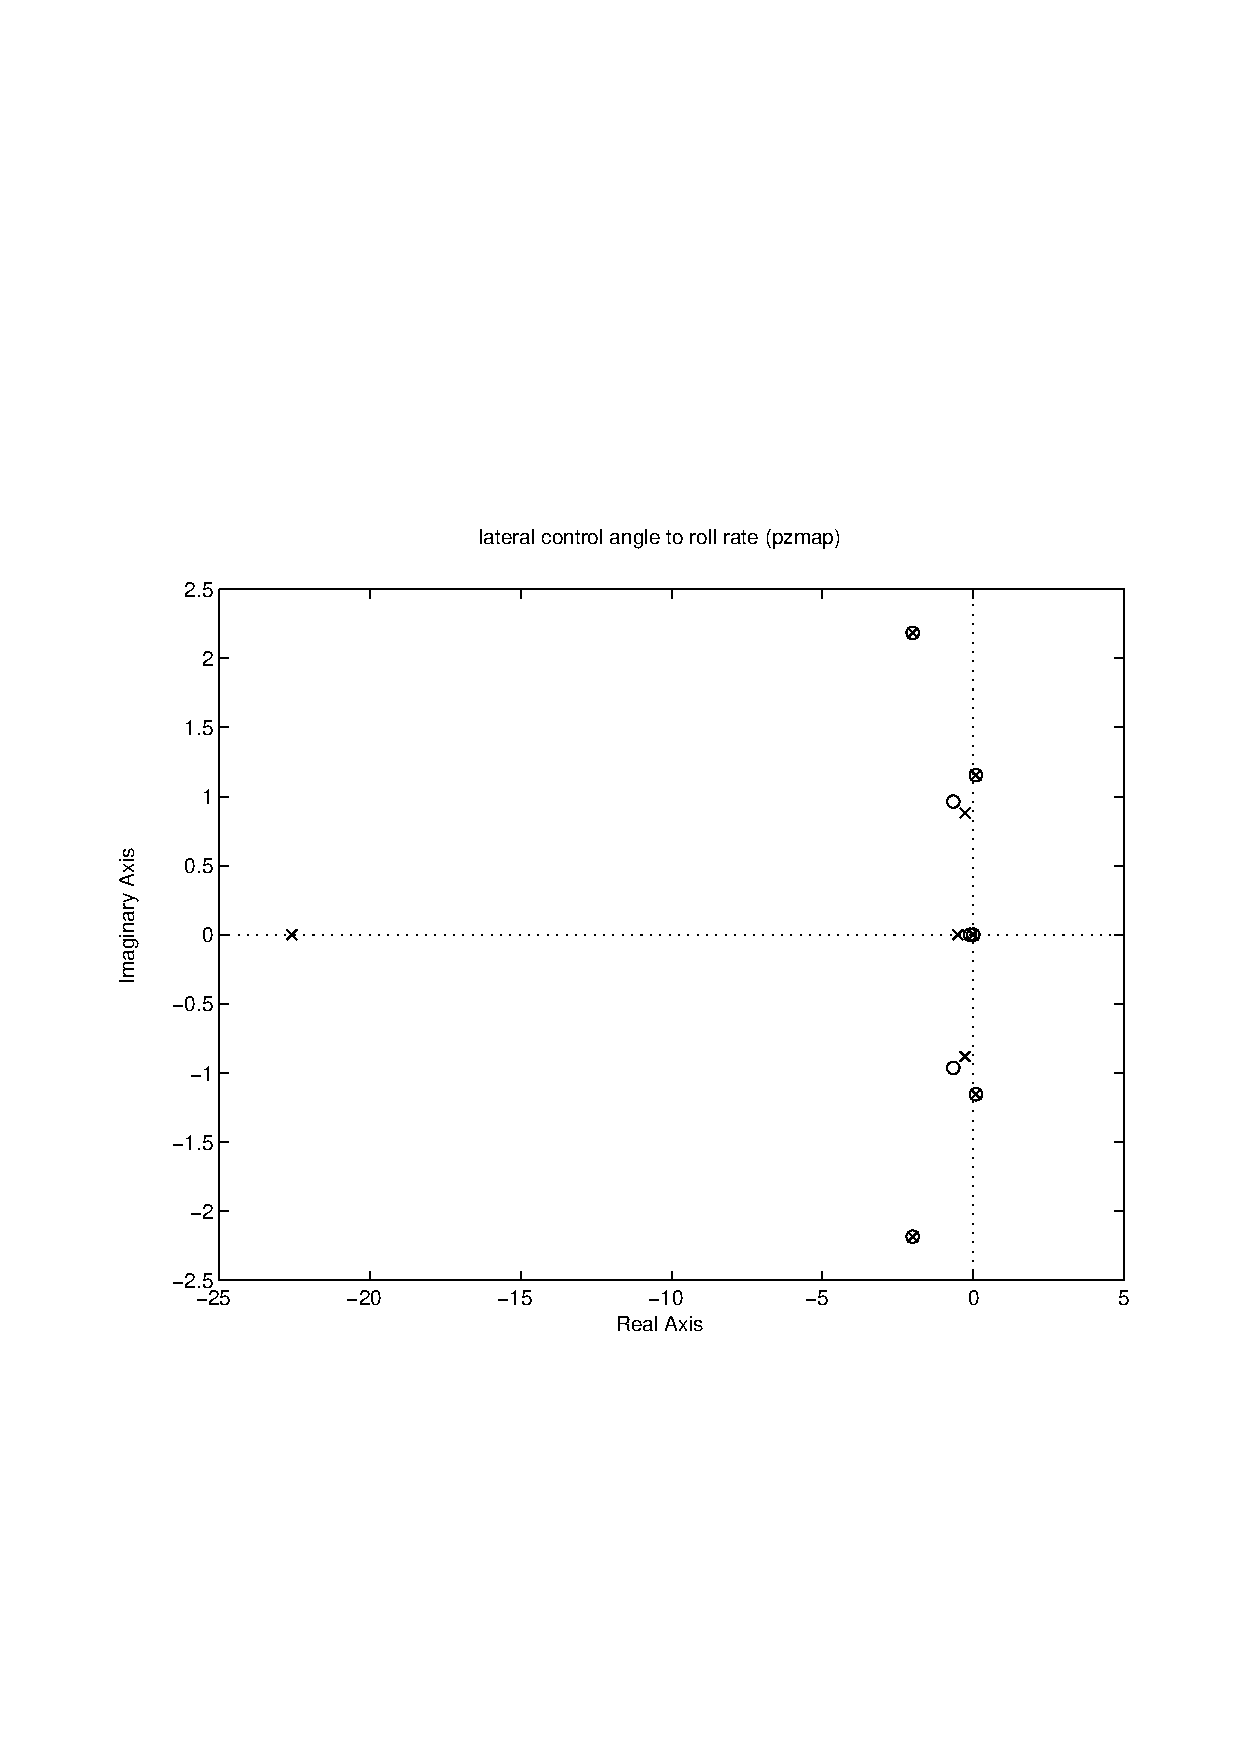
\includegraphics[width=0.8\columnwidth]{figs/26pz}
    \caption{Roll rate}
    \label{fig:lat2}
\end{figure}

\begin{figure}[h]
    \centering
    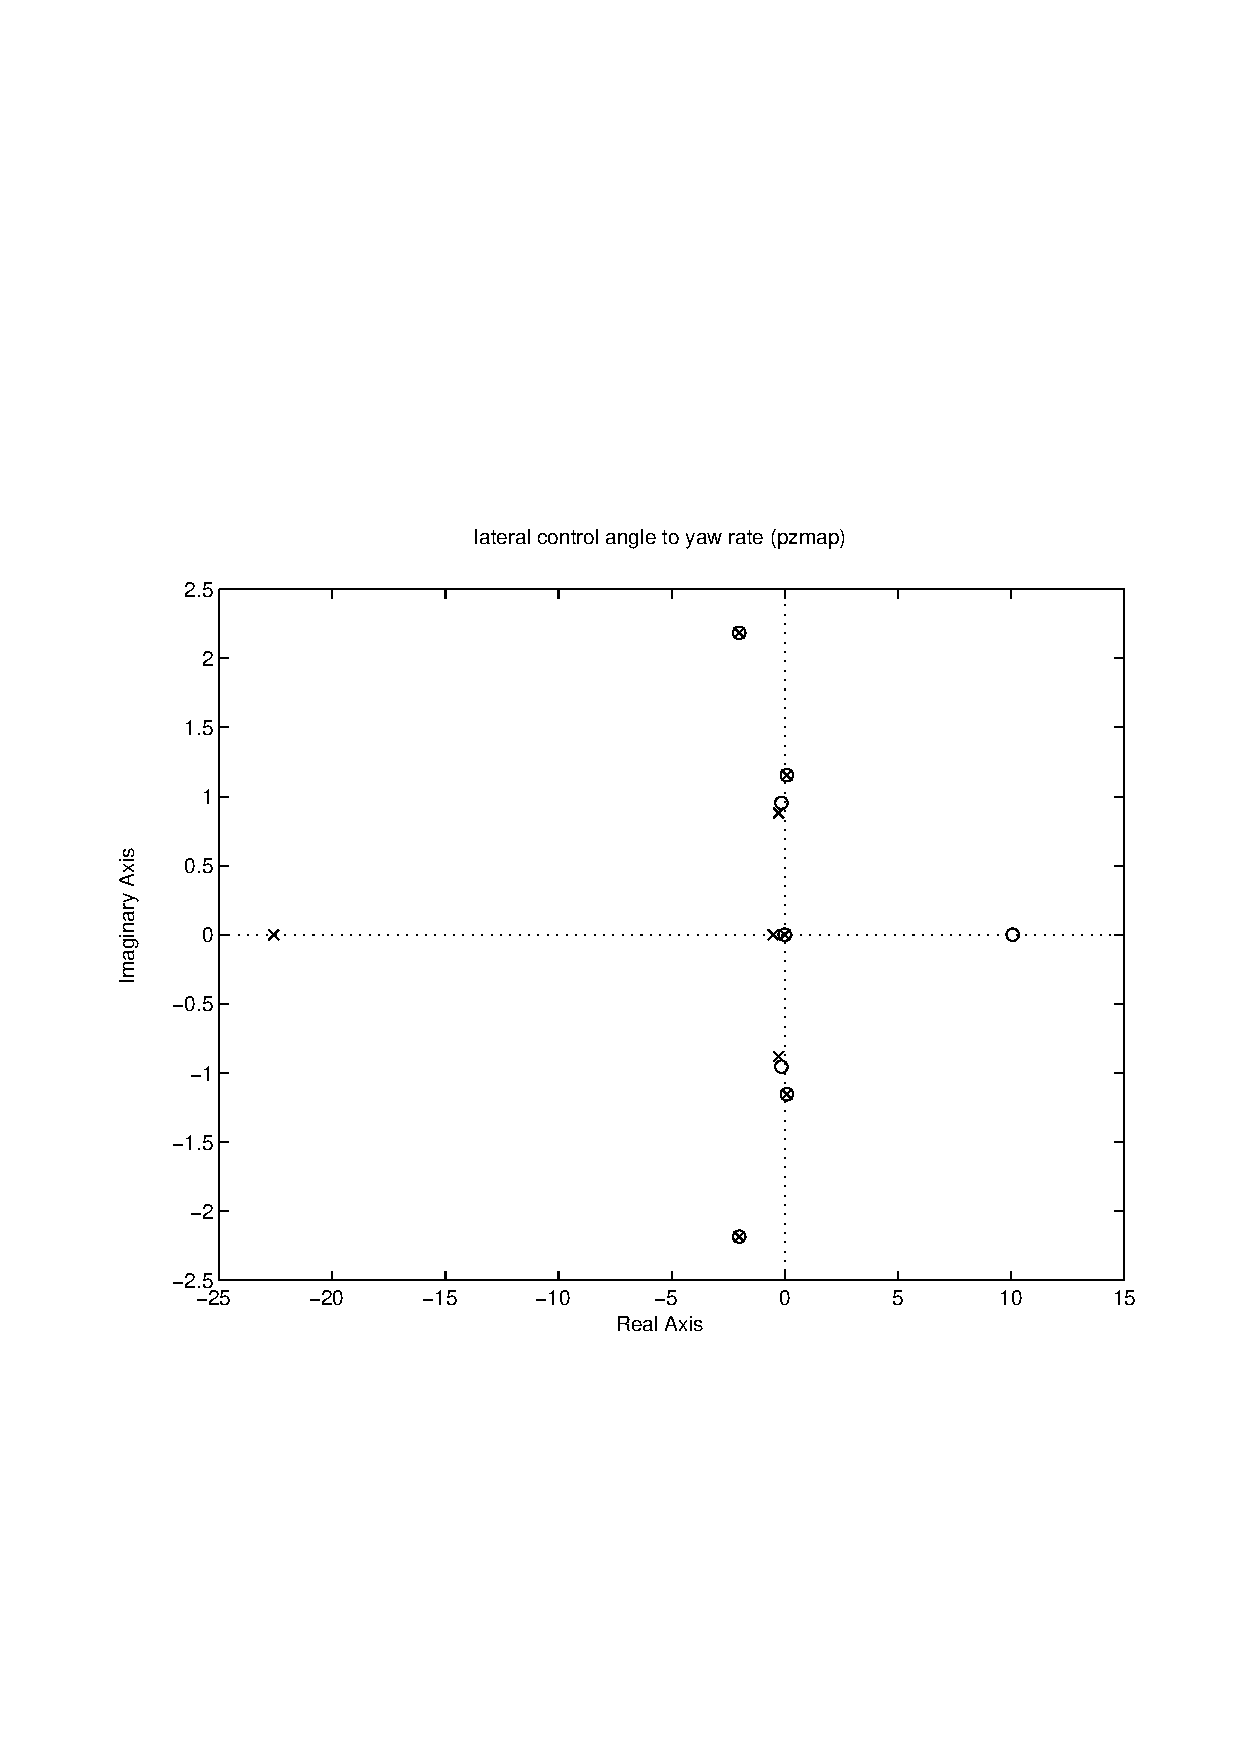
\includegraphics[width=0.8\columnwidth]{figs/27pz}
    \caption{Yaw rate}
    \label{fig:lat3}
\end{figure}

\begin{figure}[h]
    \centering
    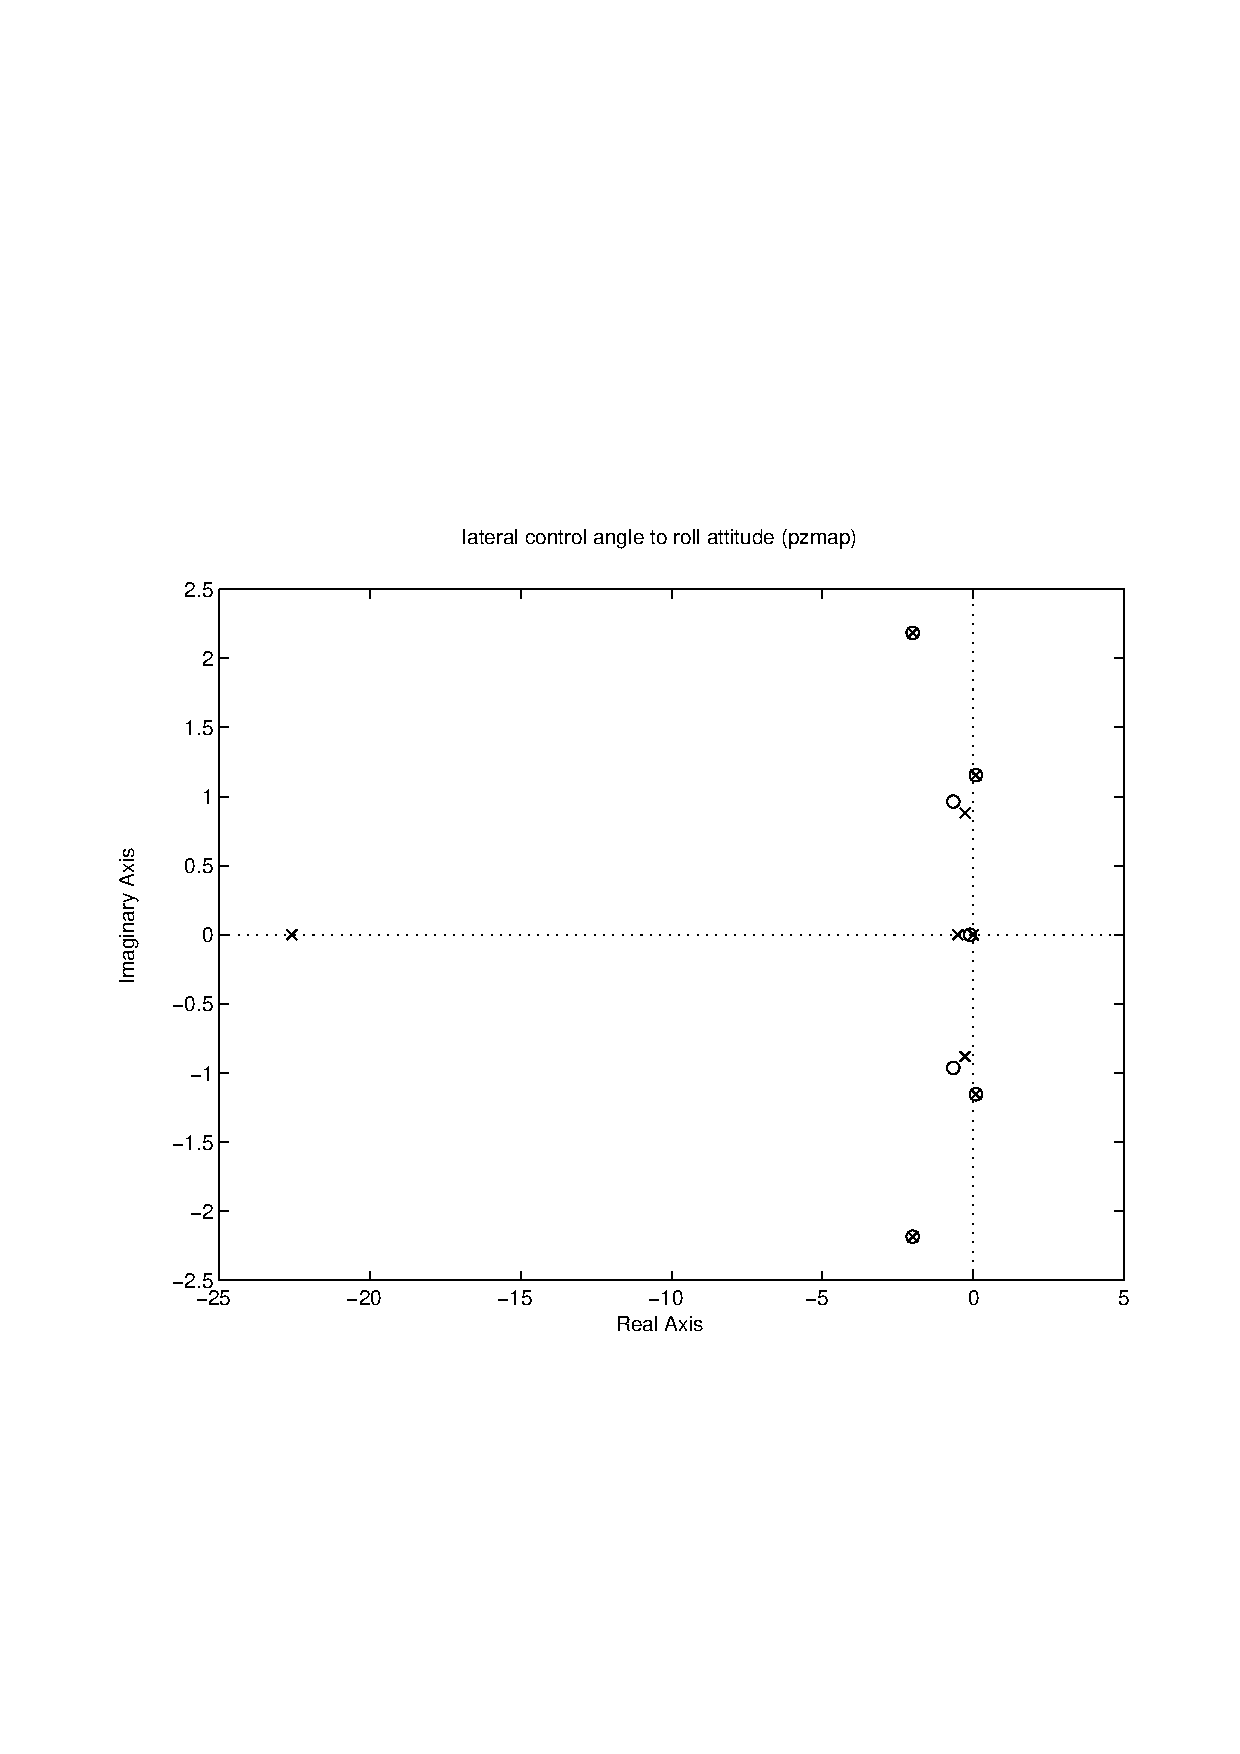
\includegraphics[width=0.8\columnwidth]{figs/28pz}
    \caption{Roll attitude}
    \label{fig:lat4}
\end{figure}

\begin{figure}[h]
    \centering
    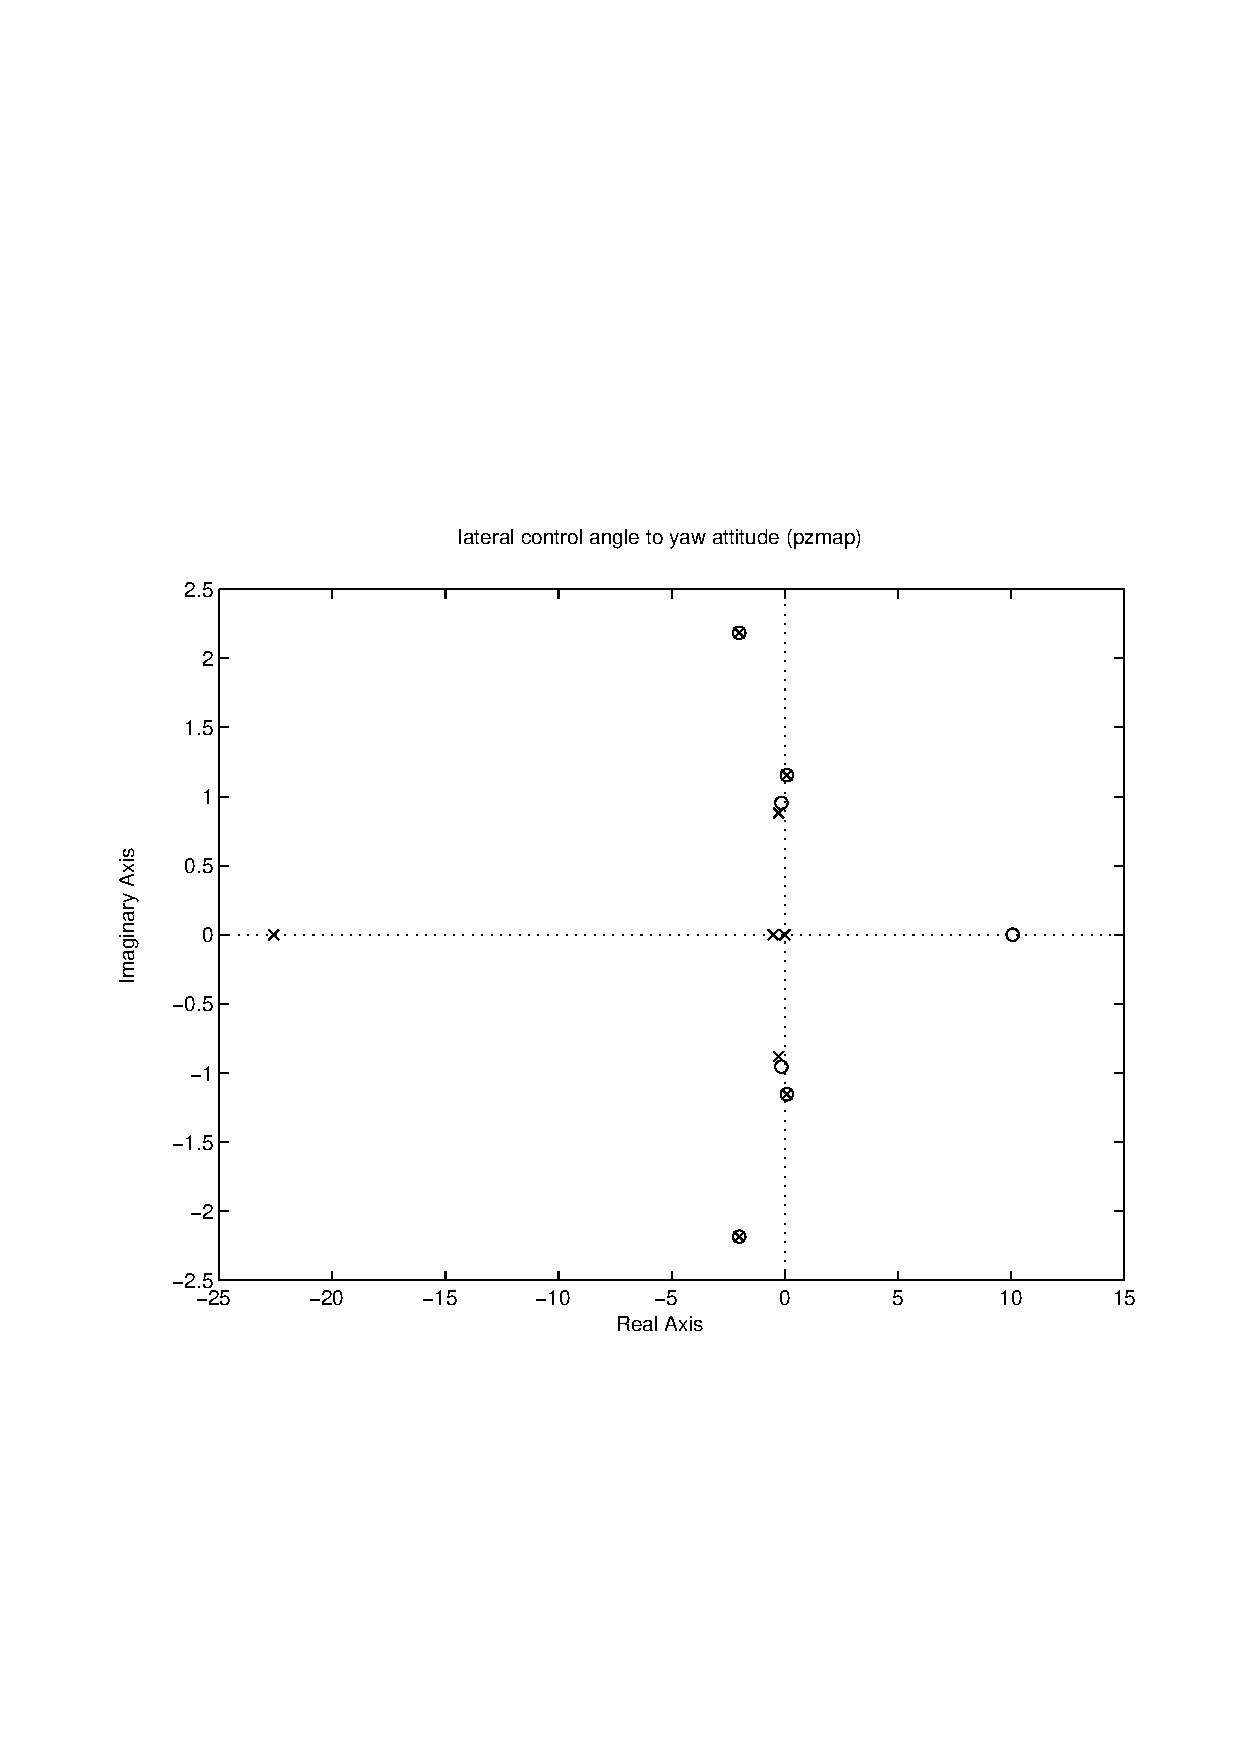
\includegraphics[width=0.8\columnwidth]{figs/29pz}
    \caption{Yaw attitude}
    \label{fig:lat5}
\end{figure}

\chapter{Final Controller Parameters}
\label{sec:ctrlvals}

\setcounter{MaxMatrixCols}{20}
\begin{align*}
    \gls{Q} &=
    \begin{bmatrix}
        1 & 0 & 0 & 0 & 0 & 0 & 0 & 0 & 0 & 0 & 0 \\
        0 & 1 & 0 & 0 & 0 & 0 & 0 & 0 & 0 & 0 & 0 \\
        0 & 0 & 1 & 0 & 0 & 0 & 0 & 0 & 0 & 0 & 0 \\
        0 & 0 & 0 & 1 & 0 & 0 & 0 & 0 & 0 & 0 & 0 \\
        0 & 0 & 0 & 0 & 1 & 0 & 0 & 0 & 0 & 0 & 0 \\
        0 & 0 & 0 & 0 & 0 & 1 & 0 & 0 & 0 & 0 & 0 \\
        0 & 0 & 0 & 0 & 0 & 0 & 1 & 0 & 0 & 0 & 0 \\
        0 & 0 & 0 & 0 & 0 & 0 & 0 & 1 & 0 & 0 & 0 \\
        0 & 0 & 0 & 0 & 0 & 0 & 0 & 0 & 1 & 0 & 0 \\
        0 & 0 & 0 & 0 & 0 & 0 & 0 & 0 & 0 & 1 & 0 \\
        0 & 0 & 0 & 0 & 0 & 0 & 0 & 0 & 0 & 0 & 600
    \end{bmatrix}
    \\
    \gls{R} &=
    \begin{bmatrix}
        50 & 0 \\
        0 & 50
    \end{bmatrix}
    \\
    \gls{K} &=
    \begin{bmatrix}
        -0.0416 & -0.0174 & 0.377 & 1.18 & 0 & 0 & 0 & 0 & 0 & 0.141 & 0 \\
        0 & 0 & 0 & 0 & -0.219 & 0.595 & 2.31 & 4.42 & 0.217 & 0 & 3.46
    \end{bmatrix}
\end{align*}

\printglossary[type=symbol]

\addcontentsline{toc}{chapter}{Bibliography}
\bibliography{syde460final}
\end{document}
